%%%%%%%%%%%%%%%%%%%%%%%%%%%%%%%%%%%%%%%%%%%%%%%%%%%%%%%%%%%%%%%%%%%%%%%%%%%%%%%%
%%                           ONDER DE LOEP ARTIKEL                            %%
%%%%%%%%%%%%%%%%%%%%%%%%%%%%%%%%%%%%%%%%%%%%%%%%%%%%%%%%%%%%%%%%%%%%%%%%%%%%%%%%

\artikelfoto{Speltheorie}{}{Michel Roelens\\ Els Vanlommel\\Luc Van den Broeck }{img/Lspeltheorie/bannerspeltheorie.jpg}

\startcontents[inhoudloep]	% om inhoud voor het loep artikel te beginnen

\begin{multicols}{2}

\inhoudstafelloep			% om inhoudstafel voor het loep artikel te tonen


\section{Inleiding}

%Een korte loep!

Speltheorie is niet zomaar theorie over spelletjes. In speltheorie zijn er twee of meer partijen die, om de beurt of tegelijkertijd, op een rationele manier keuzes maken en hiermee proberen om hun `opbrengst' (niet per se geld) te maximaliseren of hun `verlies' te minimaliseren. Speltheorie wordt veel gebruikt in situaties die we niet met spellen associëren zoals de economie, de politiek, de sport … en natuurlijk ook, zoals de naam het zegt, in de analyse van bepaalde strategische spellen. Het gaat dan niet over bijvoorbeeld ganzenbord, waarbij het spelverloop louter door het toeval wordt bepaald. De partijen worden meestal `spelers' genoemd en de keuzes die ze maken `zetten' of `acties'.

Met deze loep willen we geen cursus of lessenreeks rond speltheorie uitwerken. We kiezen voor korte voorbeelden en activiteiten die in beperkte tijd en los van elkaar aan leerlingen aangeboden kunnen worden. Sommige activiteiten kunnen aansluiten bij kansrekening in de derde graad, of zijn geschikt als tussendoortje: een uitweiding, een projectje, een deel van een lessenmarathon …

Qua voorkennis kan het ook in studierichtingen met minder wiskunde of in de tweede graad. Deze voorbeelden en activiteiten vereisen weinig algebraïsche vaardigheden. Op die manier kun je focussen op het redeneren, ook bij leerlingen die in wiskunde vaak vastlopen op het algebraïsch rekenen.

We starten in \autoref{sec:boterkaaseieren} met het spel boter-kaas-en-eieren. Dit spel eindigt, als beide spelers slim spelen, in gelijkspel. Er zijn ook spellen, zoals Nim en Chomp, die voor één van de spelers een winnende strategie hebben. Daar gaat \autoref{sec:winningstrat} over. In \autoref{sec:companiesandprisoners} bekijken we een vereenvoudigd model voor de concurrentie van bedrijven en vergelijken we dit met het beruchte dilemma van de gevangenen. \hyperref[sec:bladsteenschaar]{Paragraaf 5} gaat over het bekende spel blad-steen-schaar. Met een klassiek verhaal over de detective Sherlock Holmes hebben we het in \autoref{sec:holmes} over het Nash-evenwicht. In \autoref{sec:penalties} passen we het Nash-evenwicht toe op strafschoppen bij voetbal. Een korte paragraaf over geschiedenis van de speltheorie beëindigt deze loep. Veel leesplezier.

\section{Boter-kaas-en-eieren}\label{sec:boterkaaseieren}

In een $3\times3$-rooster plaatsen twee spelers om beurten een letter: de ene (Xeno) steeds een $\times$ en de ander (Oona) steeds een o. Wie als eerste drie gelijke letters op een rij, kolom of diagonaal heeft, wint.

Dit eenvoudige spel wordt in Engeland noughts and crosses genoemd en in Amerika tic-tac-toe.

Boter-kaas-en-eieren is een voorbeeld van een spel met twee spelers die om beurten een zet moeten doen. Het toeval speelt geen rol, maar wel de zetten van de tegenspeler.

Een interessante vraag is of één van beide spelers altijd kan winnen. Leerlingen kunnen dit eerst uitproberen. Ze zullen merken dat de speler die mag beginnen, zeg maar Xeno, kan zorgen dat hij nooit verliest. Ofwel zal Xeno winnen, ofwel wordt het gelijkspel. En als Oona ook slim speelt, dan wordt het telkens gelijkspel. Dit maakt het spel wel een beetje saai als het gespeeld wordt door twee mensen die het spel te goed kennen … We bekijken eerst een voorbeeld.

\begin{tabular}{c|c|c}
  $\times$ & \; & \; \\      \hline
   &  &  \\      \hline
   &  & 
\end{tabular}
$\rightarrow$
\begin{tabular}{c|c|c}
  $\times$ & \; & \; \\      \hline
   &  &  \\      \hline
  o &  & 
\end{tabular}
$\rightarrow$
\begin{tabular}{c|c|c}
  $\times$ & \; & \; \\      \hline
  $\times$ &  &  \\      \hline
  o &  & 
\end{tabular}

$\rightarrow$ 
\begin{tabular}{c|c|c}
  $\times$ & \; & \; \\      \hline
   $\times$&  o&  \\      \hline
  o &  & 
\end{tabular}
$\rightarrow$ 
\begin{tabular}{c|c|c}
  $\times$ & \; & $\times$ \\      \hline
   $\times$&  o&  \\      \hline
  o &  & 
\end{tabular}
$\rightarrow$
\begin{tabular}{c|c|c}
  $\times$ & o & $\times$ \\      \hline
   $\times$&  o&  \\      \hline
 o &  & 
\end{tabular}

$\rightarrow$ \begin{tabular}{c|c|c}
  $\times$ & o & $\times$ \\      \hline
   $\times$&  o&  \\      \hline
  o &  $\times$& 
\end{tabular}$\rightarrow$ 
gelijkspel.

Had Xeno nog kunnen winnen nadat de eerste $\times$ en o geplaatst waren? Ja, bijvoorbeeld door zo te spelen:

$\rightarrow$
\begin{tabular}{c|c|c}
  $\times$ & \; & $\times$ \\      \hline
   &  &  \\      \hline
  o &  & 
\end{tabular}$\rightarrow$
\begin{tabular}{c|c|c}
  $\times$ & o & $\times$ \\      \hline
   &  &  \\      \hline
  o &  & 
\end{tabular}
$\rightarrow$ 
\begin{tabular}{c|c|c}
  $\times$ & o & $\times$ \\      \hline
   &  &  \\      \hline
  o &  & $\times$
\end{tabular}

Nu kan Oona hem niet tegelijk in de derde kolom en in een diagonaal afblokken.

Om te winnen wil Xeno een situatie creëren waarbij Oona op twee plaatsen tegelijk moet verhinderen dat Xeno drie $\times$-en op een rij kan plaatsen.
Als Xeno in een hoek begint en Oona begint niet in het midden, dan kan Xeno altijd winnen. Als Oona wel haar eerste o in het midden plaatst, dan kan Xeno niet meer winnen maar kan hij wel zorgen voor gelijkspel. En als Xeno in het midden begint, kan hij zorgen voor gelijkspel. Je kunt dit aantonen door alle mogelijke `verschillende' gevallen na te gaan (verschillend rekening houdend met de symmetrie).

In de lesactiviteit beschrijven we een goocheltruc die je met boter-kaas-en-eieren kunt doen, gebaseerd op Scam Nation (s.d.). Deze goocheltruc steunt op de situatie waarbij Xeno in het midden begint en op de symmetrie van het eindresultaat.

\end{multicols}

\begin{lesactiviteit}{Boter-kaas-en-eieren: de voorspelling}

Je kunt een goocheltruc doen met boter-kaas-en-eieren. We leggen eerst uit hoe de truc werkt.

Jij speelt boter-kaas-en-eieren tegen iemand die de truc niet kent (laten we die Oona noemen). Jij speelt met $\times$ en je mag beginnen. Je zegt dat Oona een aantrekkelijke prijs krijgt als zij van je wint. Dit is belangrijk: de truc werkt immers niet als Oona zich laat verliezen (door in een rij, kolom of diagonaal met twee $\times$'en geen o te plaatsen).

Op voorhand maak je een blaadje met een voorspelling van het eindresultaat (zie verderop).

Je begint met een $\times$ in het midden. Als Oona een o in een hoek plaatst, plaats je een $\times$ in het aangrenzend vakje in tegenwijzerzin. Als Oona een o niet in een hoek plaatst, zet je een $\times$ in het aangrenzend vakje in wijzerzin. 

Hieronder een mogelijk spelverloop:\\
\resizebox{!}{0.8cm}{%
    \begin{tabular}{c|c|c}
  \; &  & \; \\      \hline
   &  $\times$&  \\      \hline
   &  & 
\end{tabular}
}$\rightarrow$
\resizebox{!}{0.8cm}{%
\begin{tabular}{c|c|c}
  \; &  & \; \\      \hline
   &  $\times$& o\\      \hline
   &  & 
\end{tabular}
}$\rightarrow$
\resizebox{!}{0.8cm}{%
\begin{tabular}{c|c|c}
  \; &  & \; \\      \hline
   &  $\times$& o \\      \hline
   &  & $\times$
\end{tabular}
}$\rightarrow$
\resizebox{!}{0.8cm}{%
\begin{tabular}{c|c|c}
  o &  & \; \\      \hline
   & $\times$& o \\      \hline
   &  & $\times$
\end{tabular}
}$\rightarrow$
\resizebox{!}{0.8cm}{%
\begin{tabular}{c|c|c}
 o &  & \; \\      \hline
  $\times$ &  $\times$& o \\      \hline
   &  & $\times$
\end{tabular}
}$\rightarrow$
\resizebox{!}{0.8cm}{%
\begin{tabular}{c|c|c}
 o &  o& \; \\      \hline
  $\times$ &  $\times$& o \\      \hline
   &  & $\times$
\end{tabular}
}

$\rightarrow$
\resizebox{!}{0.8cm}{%
\begin{tabular}{c|c|c}
 o &  o& $\times$\\      \hline
  $\times$ &  $\times$& o \\      \hline
   &  & $\times$
\end{tabular}
}$\rightarrow$
\resizebox{!}{0.8cm}{%
\begin{tabular}{c|c|c}
 o &  o& $\times$\\      \hline
  $\times$ &  $\times$& o \\      \hline
   o&  & $\times$
\end{tabular}
}$\rightarrow$
\resizebox{!}{0.8cm}{%
\begin{tabular}{c|c|c}
 o &  o& $\times$\\      \hline
  $\times$ &  $\times$& o \\      \hline
   o& $\times$ & $\times$
\end{tabular}} (*)

\begin{vraagenantwoord}
    \vraag{Noteer een ander spelverloop. Kom je hetzelfde uit op het einde?}
    
    \antwoord{Niet per se letterlijk hetzelfde als (*), maar wel op een draaiing na hetzelfde.}

    \end{vraagenantwoord}
    
In vraag 3 ga je dit voor elk mogelijk spelverloop controleren. Maar eerst leggen we verder de truc uit. 

    \begin{vraagenantwoord}[resume]
        
       \vraag{Wat moet je op voorhand als voorspelling op het blaadje schrijven?}

    \antwoord{Je noteert het resultaat (*) op het blaadje. Om dan te tonen dat je juist voorspeld had, draai je onopvallend het voorspellingsblaadje in de zelfde stand als wat je bent uitgekomen. Je zet de voorspelling best op een vierkant blaadje, zodat het niet opvalt hoe je het draait.}

%    \vraag{Je zou de voorspelling ook op een doorschijnend vierkant blaadje kunnen zetten. Wat is hiervan het voordeel?}

 %   \antwoord{Door te experimenteren kunnen de leerlingen ontdekken dat wijzerzin of tegenwijzerzin niet meer uitmaakt. Je mag telkens willekeurig een vakje kiezen aangrenzend aan de laatste o. Hieronder zie je een mogelijk spelverloop. Een nadeel van de voorspelling op transparant is dat het misschien minder spectaculair lijkt: het trekt meteen de aandacht op het aspect `op een isometrie na' \ldots}


%\emph{Je ziet dat het resultaat in dit voorbeeld niet meer op een draaiing na hetzelfde is als (*), maar op een spiegeling na (het transparante blaadje omkeren in de ruimte \ldots). Concreet moet je hier spiegelen ten opzichte van de diagonaal van linksboven naar rechtsonder. In het algemeen kan men bewijzen dat je altijd een draaibeeld of spiegelbeeld van (*) uitkomt.}

\end{vraagenantwoord}

We willen nu bewijzen dat je op een draaiing na altijd hetzelfde eindresultaat (*) verkrijgt.

\begin{vraagenantwoord}[resume]
    
\vraag{Als jij $\times$ in het midden plaatst, zijn er op een draaiing na twee mogelijkheden voor de eerste zet van Oona. Leg uit.}

\antwoord{Zij kan een o in een hoek plaatsen of niet in een hoek. Alle mogelijkheden met een $\times$ in het midden en één $o$ in een hoek zijn op draaiing na hetzelfde en idem met één $o$ niet in een hoek.}

\vraag{Onderzoek alle mogelijke spelverlopen. Verdeel het werk: de helft van de klas neemt de eerste mogelijkheid voor de eerste zet van Oona en de andere helft van de klas neemt de tweede. Voor jou als $\times$-speler is er nooit keuze. Je volgt de regel over wijzerzin of tegenwijzerzin. Voor Oona is er ook geen keuze wanneer ze twee $\times$-en en een leeg vakje op een rij, kolom of diagonaal krijgt; dan moet ze afblokken. Maar als dat niet het geval is, kan zij kiezen en moet je alle gevallen nakijken.}

\antwoord{We bekijken het geval waarbij Oona haar eerste o in een hoek plaatst. Het andere geval is analoog.}

    \begin{tabular}{c|c|c}
  \; &  & o \\      \hline
   &  $\times$&  \\      \hline
   &  & 
\end{tabular}
$\xrightarrow{\text{tegenwijzerzin}}$
    \begin{tabular}{c|c|c}
  \; & $\times$ & o \\      \hline
   &  $\times$&  \\      \hline
   &  & 
\end{tabular}
$\xrightarrow{\text{afblokken}}$
 \begin{tabular}{c|c|c}
  \; & $\times$ & o \\      \hline
   &  $\times$&  \\      \hline
   &  o& 
\end{tabular}
$\xrightarrow{\text{wijzerzin}}$
 \begin{tabular}{c|c|c}
  \; & $\times$ & o \\      \hline
   &  $\times$&  \\      \hline
  $\times$ &  o& 
\end{tabular}
(**)

\emph{Vanaf (**) zijn er voor Oona vier mogelijkheden; we bekijken het vakje linksboven.}

\begin{tabular}{c|c|c}
  o & $\times$ & o \\      \hline
   &  $\times$&  \\      \hline
  $\times$ &  o& 
\end{tabular}
$\xrightarrow{\text{tegenwijzerzin}}$
\begin{tabular}{c|c|c}
  o & $\times$ & o \\      \hline
  $\times$ &  $\times$&  \\      \hline
  $\times$ &  o& 
\end{tabular}
$\xrightarrow{\text{afblokken}}$
\begin{tabular}{c|c|c}
  o & $\times$ & o \\      \hline
  $\times$ &  $\times$& o \\      \hline
  $\times$ &  o& 
\end{tabular}
$\xrightarrow{\text{wijzerzin}}$
\begin{tabular}{c|c|c}
  o & $\times$ & o \\      \hline
  $\times$ &  $\times$& o \\      \hline
  $\times$ &  o& $\times$
\end{tabular}


\emph{Om te tonen dat dit hetzelfde resultaat is als op het voorspellingsblaadje, moet je het blaadje met (*) erop over 90° in wijzerzin draaien.}

\emph{De verdere spelverlopen bij de drie andere mogelijkheden vanaf (**) zijn analoog. De klas kan misschien op een groot blad een boom maken waarin ze alle spelverlopen samenbrengen: bovenaan twee hoofdtakken die zich een beetje lager bij (**) elk in vier deeltakken verdelen. Dit geeft onderaan acht eindresultaten, niet allemaal verschillend, die alle acht op een draaiing na gelijk zijn aan het eindresultaat (*) dat op het blaadje staat.}

\end{vraagenantwoord}

\end{lesactiviteit}\clearpage

\begin{multicols}{2}

%Wat kan er nog met OXO? Telproblemen: op hoeveel mogelijke manieren kun je het $3\times 3$-rooster invullen met 5 keer een X en 4 keer een O (ja: de speler die begint speelt één keer meer \ldots)? Dat is niet zo moeilijk: het aantal combinaties van 5 (of van 4) uit 9, dat is $C^5_9=126$. Maar hoeveel verschillende manieren zijn er op draaiing na? En als je ze ook mag spiegelen zoals met het transparant in de vorige lesactiviteit? Het antwoord is 23, maar dat is wel even puzzelen, tenzij voor wie op de hoogte is van een stukje hogere wiskunde: de stelling van Burnside , die Luc ons uitgelegd heeft in de loep over teltechnieken, Uitwiskeling 35/3 \ldots

%Misschien is OXO ook een geschikte context om leerlingen te laten programmeren, bv. in Python. ((Mij goed zolang ze het niet aan mij komen vragen \ldots))
    

\section{Winnende strategieën}\label{sec:winningstrat}
\subsection*{Nim}
Het spelletje boter-kaas-en-eieren is uit wiskundig oogpunt een vrij saai spel. Het is een eindig spel waarbij er slechts een beperkt aantal manieren bestaat om het spel te laten verlopen. Dat merk je al als je berekent op hoeveel manieren je 9 vakjes kunt vullen met een o, met een $\times$ of met niets. Zonder rekening te houden met de symmetrie van de  bordvullingen zijn dat $3^9$ mogelijkheden. Maar dit getal is een sterke overschatting van het aantal mogelijke eindposities want de eindposities met bijvoorbeeld meer o's dan $\times$'en zijn verboden. En eindposities met meerdere series van drie gelijke tekens op een rij ook. Buiten de beperktheid van het aantal eindsituaties, is er nog een andere storende factor. Als beide spelers alle mogelijke inzichten benutten, is er geen van de spelers die een overwinning kan afdwingen. Saai dus. 

In deze paragraaf zullen we het enkel hebben over eindige strategische spellen waarbij er geen gelijkspel mogelijk is. Eén van deze spelletjes is het nimspel, waarvan er talrijke varianten bestaan. Hieronder zie je de spelregels van de meest gebruikelijke variant.

\begin{quote}
    Op tafel ligt een stapel lucifers. Beide spelers nemen om beurt één of twee lucifers weg. Wie de laatste lucifer wegneemt, is verloren.
\end{quote}

Ook dit spel is redelijk voorspelbaar als je de wiskundige analyse gemaakt hebt. Stel dat \textcolor{red}{rood} tegen \textcolor{green}{groen} speelt en dat \textcolor{red}{rood} als eerste aan zet is. Dan bestaat er een \emph{winnende strategie} voor \textcolor{red}{rood} als het aantal lucifers op de stapel niet een drievoud plus één is. Deze strategie bestaat er in bij de eerste zet één of twee lucifers weg te nemen tot er een drievoud plus één overblijft. Wat \textcolor{green}{groen} nu ook onderneemt,  \textcolor{red}{rood} kan er altijd voor zorgen dat er na zijn beurt een drievoud plus één overblijft. Als \textcolor{green}{groen} er één neemt, neemt \textcolor{red}{rood} er twee. Als \textcolor{green}{groen} er twee neemt, neemt \textcolor{red}{rood} er één. 

Het is duidelijk dat een drievoud plus één een winnende spelpositie is. \textcolor{green}{Groen} kan hier niet uit ontsnappen. Omdat het aantal overblijvende lucifers na elke beurt daalt, laat \textcolor{red}{rood} na een eindig aantal zetten één (het kleinste drievoud plus één) lucifer achter. Hiermee verzekert hij zich van de overwinning.

Als het aantal lucifers bij het begin van het spel wel een drievoud plus één is, dan bestaat er een winnende strategie voor \textcolor{green}{groen}. Je komt er vast zelf wel achter hoe deze strategie werkt.


\subsection*{Zijn er altijd winnende strategieën?}
Het voorbeeld van het nimspel suggereert dat er voor spellen zonder gelijkspel (remise, ex aequo, draw)  altijd een winnende strategie is ofwel voor \textcolor{red}{rood} (de speler die de eerste zet doet) ofwel voor \textcolor{green}{groen} (de speler die het laatst aan zet komt). Dit is inderdaad het geval, maar alleen als het spel eindig is. We tonen dit hieronder aan door te steunen op enkele wetten uit de logica: de wet van de uitgesloten derde en de wet van De Morgan. 

We formaliseren hiervoor eerst de uitspraak dat er een winnende strategie is voor \textcolor{red}{rood}. Dit betekent dat er een eerste zet \textcolor{red}{$x_1$} voor \textcolor{red}{rood} bestaat, zo dat voor elke eerste zet \textcolor{green}{$y_1$}  van \textcolor{green}{groen} er een tweede zet \textcolor{red}{$x_2$} voor \textcolor{red}{rood} bestaat, zo dat voor elke tweede zet \textcolor{green}{$y_2$} van \textcolor{green}{groen} geldt … zo dat \textcolor{red}{rood} wint. Met kwantoren ($\forall$ en $\exists$) kunnen we dit zeer bondig noteren.
\[ \textcolor{red}{\exists x_1} \; \textcolor{green}{\forall y_1} \; \textcolor{red}{\exists x_2} \; \textcolor{green}{\forall y_2}  \;  \textcolor{red}{\exists x_3} \; \textcolor{green}{\forall y_3} \;\cdots \;  \textcolor{red}{\textrm{rood wint}}\]

Ofwel is de uitspraak hierboven waar ofwel is ze onwaar. Dat is de wet van de uitgesloten derde. Als deze uitspraak onwaar is, dan geldt via de wet over de negatie van kwantoren dat
\[ \textcolor{red}{\forall x_1} \; \textcolor{green}{\exists y_1} \; \textcolor{red}{\forall x_2} \; \textcolor{green}{\exists y_2}  \;  \textcolor{red}{\forall x_3} \; \textcolor{green}{\exists y_3} \;\cdots \; \textcolor{red}{\textrm{rood wint niet}}\]
wat door het ontbreken van ex aequo's evenwaardig is met
\[ \textcolor{red}{\forall x_1} \; \textcolor{green}{\exists y_1} \; \textcolor{red}{\forall x_2} \; \textcolor{green}{\exists y_2}  \;  \textcolor{red}{\forall x_3} \; \textcolor{green}{\exists y_3} \;\cdots \; \textcolor{green}{\textrm{groen wint}}\]

We vatten deze redenering als volgt samen: bij eindige spellen zonder ex aequo's is er altijd ofwel een winnende strategie voor \textcolor{red}{rood} ofwel een winnende strategie voor \textcolor{green}{groen}. 

Om misverstanden uit de weg te ruimen, deze conclusie betekent natuurlijk niet dat er geen winnende strategieën kunnen bestaan voor spelletjes die ex aequo's toelaten. Een voorbeeld hiervan is \emph{Vier op een rij}, een spel waarbij de spelers om beurt een gekleurde schijf in een verticaal rooster van $6\times7$ gaatjes laten zakken met de bedoeling vier gelijkgekleurde schijven aaneensluitend op een rij, een kolom of een diagonaal te krijgen. Als het rooster helemaal vol is zonder een vier op een rij, dan is het gelijkspel. In de numberphileclip \href{https://www.youtube.com/watch?v=yDWPi1pZ0Po}{Connect Four} verneem je dat er in totaal $\num{4531985219092}$ manieren zijn om het spel uit te spelen. Er blijkt ook een winnende strategie te zijn voor wie eerst aan zet is. Hij of zij moet de eerste schijf in de middelste kolom droppen.

\subsection*{Chomp}
Misschien vraag je je nu af waarom het nog de moeite is om eindige spellen zonder ex aequo's te spelen. Het staat immers in de sterren geschreven wie er zal winnen als beide partijen verstandig genoeg zijn. Het antwoord hierop is eenvoudig. Bij vele van deze spellen is de winnende strategie ons niet bekend omdat het aantal mogelijke spelsituaties en het aantal mogelijke spelverlopen onhandelbaar groot is. 

Het zal je wellicht verbazen dat er spellen zijn waarbij de partij met de winnende strategie gekend is zonder dat de mensheid iets kan zeggen over de winnende strategie. Eén van deze spellen is Chomp, een Russische roulette-spel voor chocolade-eters. Ziehier de spelregels.

\begin{quote}
Neem een rechthoekig stuk chocolade dat verdeeld is in $m\times n$ vierkante blokjes. Het blokje linksboven $b_{11}$ is vergiftigd. Wie dit opeet, verliest het spel. Om beurt breken de twee spelers een stuk chocolade van de rechthoek af volgens deze  regel. De speler wijst een blokje $b_{ij}$ aan en eet dit op samen met alle blokjes die er nog resten van de rechthoek met als linkerbovenhoek blokje $b_{ij}$ en met rechteronderhoek blokje  $b_{mn}$.
\end{quote}

In \autoref{chomp} zie je een eenvoudig spelverloop met een rechthoek van $4\times 5$ blokjes. Na  4 zetten moet de beginner, speler \textcolor{red}{rood}, het vergiftigde stukje nemen.

\afbeelding[8cm]{img/Lspeltheorie/chomp.png}{Een eenvoudig spelverloop}{chomp}

Het spel Chomp is duidelijk een spel met een eindig aantal zetten. Er zijn geen ex aequo's: er is slechts één speler die mag sterven door het consumeren van een vergiftigd blokje chocolade. 

\textcolor{red}{Rood} heeft het hierboven niet goed aangepakt. Nochtans blijkt er wel een winnende strategie te bestaan voor \textcolor{red}{rood}. Niemand kent deze strategie echter voor een chocoladerechthoek van een willekeurige grootte. 

Dat deze strategie bestaat, kunnen we in enkele zinnetjes aantonen. Ofwel is er een winnende strategie voor \textcolor{red}{rood}, ofwel is er een voor \textcolor{green}{groen}. Dat toonden we eerder al aan. De laatste optie is echter onmogelijk. Stel immers dat de winnende strategie voor \textcolor{green}{groen} bestaat dan heeft \textcolor{green}{groen} een winnende repliek op elke eerste zet van \textcolor{red}{rood}, dus ook op de keuze van blokje $b_{mn}$ door \textcolor{red}{rood}. Stel dat deze winnende repliek voor \textcolor{green}{groen} er in bestaat om in de eerste zet blokje $b_{rs}$ te kiezen dan had \textcolor{red}{rood} ook in de eerste zet blokje $b_{rs}$ kunnen kiezen en dan was hij hiermee gewonnen. We noemen deze techniek \emph{strategieroof} (Eng: strategy stealing). Strategieroof lijkt ethisch een weinig hoogstaande praktijk, maar speltheoretisch heeft niemand hier een bezwaar tegen.

\subsection*{Na-aperij}

De reputatie van na-aperij is wellicht bijna even kwalijk als die van strategieroof. Toch geeft deze techniek soms zekerheid om te overwinnen. 

Stel bijvoorbeeld dat je Chomp speelt met een vierkante chocoladerechthoek. In dit geval is de winnende strategie voor \textcolor{red}{rood} wél gekend. De winnende strategie steunt op na-aperij. De beginner, \textcolor{red}{rood} dus, kiest eerst voor blokje $b_{22}$. De chocolade die hij voor \textcolor{green}{groen} nalaat is van de volgende vorm. 

\afbeelding[2cm]{img/Lspeltheorie/chomp2.jpg}{Chomp met een vierkant stuk chocolade}{chomp2}

Vervolgens heeft \textcolor{green}{groen} de keuze om een aantal blokjes af te breken van de horizontale rij of van de verticale kolom die overblijft. Speler \textcolor{red}{rood} aapt hem na bij de overgebleven arm. Zo herstelt hij het evenwicht en blijven beide armen even lang. Als beide armen opgegeten zijn, rest enkel het vergiftigde blokje voor \textcolor{green}{groen}.

Om volledig te zijn: de winnende strategie voor \textcolor{red}{rood} is ook bekend voor een chocoladerechthoek van $2 \times n$. Ook hier lukt het met na-apen om het evenwicht te herstellen. Meer hoeven we je hierover natuurlijk niet te vertellen om je aan het denken te zetten.\clearpage

\section{Bedrijven en gevangenen}\label{sec:companiesandprisoners}

\subsection{Bedrijven in concurrentie}

Speltheorie gaat niet enkel over spelletjes. In de lesactiviteit hieronder tonen we een eenvoudig voorbeeld van speltheorie in een (sterk vereenvoudigde) economische context (naar: Mr. Chadd, s.d.). Er komt een matrix in voor, maar er is geen enkele kennis van matrixrekenen nodig.
\end{multicols}

\begin{lesactiviteit}{Prijsdaling?}

Twee grote computerbedrijven, \textcolor{green}{Peer} en \textcolor{purple}{Kleinzacht}, overwegen om de prijs van hun besturingssysteem te laten dalen. Of dit interessant is, hangt af van wat hun concurrent zal doen. 

Ook al vinden ze hun handel wellicht bittere ernst, in de speltheorie worden de twee bedrijven \emph{spelers} genoemd. De keuzes die ze kunnen maken zijn \emph{zetten} of \emph{acties}.

De opbrengsten van beide spelers, afhankelijk van hun acties en die van de tegenspeler, worden voorgesteld in een tabel. Omdat er op elke plaats in de tabel twee getallen staan, de opbrengst van \textcolor{green}{Peer} vóór de puntkomma en de opbrengst voor \textcolor{purple}{Kleinzacht} erachter, noemt men die tabel een \emph{bimatrix}. De eerste speler, \textcolor{green}{Peer}, is de \emph{rijspeler}: zijn actie bepaalt in welke rij van de bimatrix we zijn opbrengsten vinden. De tweede speler, \textcolor{purple}{Kleinzacht}, is de \emph{kolomspeler}. 
  
     \begin{center}
         
    \renewcommand{\arraystretch}{1.5}
    \begin{tabular}{c c c}
        & \multicolumn{2}{c}{\textbf{\textcolor{purple}{\;\;\;\;\;\;\;\;\;\;\;\;\;\;\;\;\;\; Kleinzacht}}} \\
        & \multicolumn{1}{l}{} &  
        \begin{tabular}{cc}
            \text{prijsdaling} & \text{geen prijsdaling}
        \end{tabular} \\

        \textbf{\textcolor{green}{Peer}} &  
        $\begin{array}{c} \text{prijsdaling} \\ \text{geen prijsdaling} \end{array}$ &
        $\left[
        \begin{array}{cc}
            \textcolor{green}{2000}; \textcolor{purple}{2800}  & \textcolor{green}{2400}; \textcolor{purple}{2600}  \\
            \textcolor{green}{1800}; \textcolor{purple}{3200}  & \textcolor{green}{2200}; \textcolor{purple}{3000}  
        \end{array}
        \right]$ \\
    \end{tabular}
    \end{center}
 
De getallen in de bimatrix mag je met een korrel zout nemen; het zijn bedragen in een fictieve munteenheid.

\begin{vraagenantwoord}

\vraag{Wat is de betekenis van de getallen \textcolor{green}{2000} en \textcolor{purple}{2600} in de bimatrix?}

\antwoord{Als \textcolor{green}{Peer} zijn prijs laat zakken en \textcolor{purple}{Kleinzacht} ook, dan is de opbrengst voor \textcolor{green}{Peer} $2000$ eenheden. Als \textcolor{green}{Peer} zijn prijs laat zakken maar \textcolor{purple}{Kleinzacht} niet, dan is de opbrengst voor \textcolor{purple}{Kleinzacht} $2600$ eenheden.}

\vraag{Leg uit waarom het economisch klopt dat de grootste/kleinste opbrengsten voor een bedrijf staan waar ze staan in de bimatrix.}
\antwoord{De grootste opbrengst voor \textcolor{green}{Peer} is \textcolor{green}{$2400$} eenheden. Dit is de opbrengst als het als enige zijn prijs laat dalen: wellicht zullen er dan klanten van het andere bedrijf overkomen. De grootste opbrengst voor \textcolor{purple}{Kleinzacht}, \textcolor{purple}{$3200$}, hoort om dezelfde reden bij het geval dat \textcolor{purple}{Kleinzacht} als enige zijn prijs laat dalen. Analoog voor de laagste opbrengsten: als een bedrijf als enige zijn prijs niet laat zakken, verliest het veel klanten.}

\vraag{Is het te verwachten dat de bedrijven minder opbrengst hebben als ze allebei hun prijs laten zakken dan als ze allebei hun prijs niet laten zakken?}

\antwoord{Ja: als ze allebei hun prijs laten dalen, behouden ze hun klanten maar die betalen minder dan als de prijzen niet dalen.}
\clearpage
\vraag{Stel je in de plaats van \textcolor{green}{Peer}. Je weet niet wat \textcolor{purple}{Kleinzacht} zal beslissen. Daarom ga je uit van het voor jou ergste geval. Wat ga je doen?}

\antwoord{Ik zou de prijs laten zakken. Immers, als ik mijn prijs laat zakken, heb ik in het ergste geval een opbrengst van  \textcolor{green}{$2000$}, terwijl ik een opbrengst van slechts \textcolor{green}{$1800$} riskeer als ik mijn prijs niet laat zakken.}

\vraag{Zelfde vraag maar stel je nu in de plaats van \textcolor{purple}{Kleinzacht}.}

\antwoord{Analoog: ik zou ook mijn prijs laten dalen want dan verdien ik in het ergste geval \textcolor{purple}{$2800$}, wat meer is dan \textcolor{purple}{$2600$} wanneer ik mijn prijs niet laat zakken.}

\vraag{Wat gaan beide bedrijven doen als ze niet met elkaar afspreken?}

\antwoord{Ze gaan hun prijs laten zakken.}

\vraag{Wat zou je doen als je vooraf met het andere bedrijf kunt afspreken (en als beide bedrijven elkaar kunnen vertrouwen)?}

\antwoord{Ik zou afspreken dat geen van beide de prijs verlaagt. Dat brengt voor beide bedrijven meer op \emph{(\textcolor{green}{$2200$}, \textcolor{purple}{$3000$})} dan wat er vermoedelijk zal gebeuren zonder met elkaar af te spreken \emph{(\textcolor{green}{$2000$}, \textcolor{purple}{$2800$})}.}

\vraag{Breng dit in verband met begrippen uit de economie: het belang van concurrentie voor de consument, prijsafspraken, prijskartel … Als je zelf weinig of niets van economie af weet, spreek hier eens over met een medeleerling die in een economische studierichting zit.}

\end{vraagenantwoord}

Uiteraard is het hele verhaal sterk vereenvoudigd. Niet alleen is onduidelijk wat die opbrengsten precies zijn, maar in werkelijkheid kunnen er meer dan twee concurrerende bedrijven zijn en maakt het wellicht uit met hoeveel de prijs verlaagd wordt. 

\end{lesactiviteit}

\begin{multicols}{2}

Na deze lesactiviteit kan de leraar eventueel dit voorbeeld aangrijpen om het begrip `maximin'-strategie aan te brengen. Een andere mogelijkheid is de gelijkenis te tonen tussen dit voorbeeld en het beruchte dilemma van de gevangenen. 

\subsection{Maximinstrategie}

In de vorige lesactiviteit pasten beide spelers een \emph{maximin}-stategie toe.  

\begin{kader}{}{Maximinstrategie}

De rijspeler kijkt in zijn eigen deel van de bimatrix naar de minima in elke rij. Hij kiest de rij (de actie) die hoort bij het maximum van deze minima.

De kolomspeler kijkt in zijn eigen deel van de bimatrix naar de minima in elke kolom. Hij kiest de kolom (de actie) die hoort bij het maximum van deze minima.

\end{kader}

\vfill\null
\columnbreak

Toegepast op \textcolor{green}{Peer}: met prijsdaling van \textcolor{green}{Peer} is de minimale opbrengst \textcolor{green}{2000} en zonder prijsdaling  van \textcolor{green}{Peer} is de minimale opbrengst \textcolor{green}{1800}. Het maximum van deze minima is \textcolor{green}{2000} en daarom zal \textcolor{green}{Peer} de actie prijsdaling kiezen (de eerste rij).
Voor \textcolor{purple}{Kleinzacht} zijn de minimale opbrengsten \textcolor{purple}{2800} en \textcolor{purple}{2600}; het maximum hiervan is \textcolor{purple}{2800} en daarom kiest ook \textcolor{purple}{Kleinzacht} voor prijsdaling.

Puur voor de leerkrachten: er bestaat bij het probleem van de prijsdalingen nog een andere redenering om tot dezelfde beslissing te komen. \textcolor{green}{Peer} kan ook denken: ``als \textcolor{purple}{Kleinzacht} zijn prijs niet verlaagt, verdien ik er meer aan als ik mijn prijs wel laat zakken want \textcolor{green}{$2400$}>\textcolor{green}{$2200$}; en als \textcolor{purple}{Kleinzacht} zijn prijs wel verlaagt, is het voor mij ook interessanter om mijn prijs te verlagen want \textcolor{green}{$2000$}>\textcolor{green}{$1800$}''.
In plaats van de eigen minima per rij te vergelijken (maximin-strategie), vergelijkt \textcolor{green}{Peer} dan zijn opbrengsten per kolom en dat voor elke mogelijke actie van de tegenspeler. Op een analoge manier kan \textcolor{purple}{Kleinzacht} zijn opbrengsten per rij vergelijken. Deze redenering hoort bij het zoeken naar een zogenaamd \emph{Nash-evenwicht} (zie \autoref{sec:holmes}).
\clearpage

\subsection{Het dilemma van de gevangenen}

Opmerkelijk bij het vorige voorbeeld was dat beide spelers kiezen voor prijsverlaging terwijl het voor allebei interessanter zou zijn als ze hun prijzen niet verlagen. Als ze kunnen afspreken en elkaar vertrouwen, komt een betere uitkomst uit de bus.

Dit is hetzelfde fenomeen als in een gekend dilemma. Er zijn verschillende versies; we baseren ons hier op van Damme (1995).

\begin{quote}
    
Twee personen worden ervan verdacht gezamenlijk een moord te hebben gepleegd. Daarvoor kunnen ze elk een gevangenisstraf van 10 jaar krijgen. Ze zijn in voorlopige hechtenis genomen en gescheiden opgesloten, zo dat ze niet met elkaar kunnen communiceren. De procureur heeft nog geen sluitend bewijs. Zonder aanvullend bewijs kan elke verdachte slechts voor een kleiner vergrijp (bijvoorbeeld verboden wapendracht) veroordeeld worden, met een maximale gevangenisstraf van 1 jaar. De procureur biedt aan om een verdachte die als enige bekent, vrij te laten [waarbij de andere de maximale straf van 10 jaar krijgt]. Als beide verdachten bekennen, krijgen ze een strafvermindering van 2 jaar als beloning voor de samenwerking.

\end{quote}

De bimatrix ziet er zo uit:

 \begin{center}
         
    \renewcommand{\arraystretch}{1.5}
    \begin{tabular}{c c c}
        & \multicolumn{2}{c}{\textbf{\textcolor{purple}{\;\;\;\;\;\;\;\;\;\;\;\;\;\;\;\;\;\;\;\;verdachte 2}}} \\
        & \multicolumn{1}{l}{} &  
        \begin{tabular}{cc}
            \text{bekent} & \text{ontkent}
        \end{tabular} \\

        \textbf{\textcolor{green}{verdachte 1}} &  
        $\begin{array}{c} \text{bekent} \\ \text{ontkent} \end{array}$ &
        $\left[
        \begin{array}{cc}
            \textcolor{green}{8}; \textcolor{purple}{8}  & \textcolor{green}{0}; \textcolor{purple}{10}  \\
            \textcolor{green}{10}; \textcolor{purple}{0}  & \textcolor{green}{1}; \textcolor{purple}{1}  
        \end{array}
        \right]$ \\
    \end{tabular}
    \end{center}

Merk op dat er nu geen opbrengsten maar straffen in de bimatrix staan. Beide spelers willen hun straf niet maximaliseren maar minimaliseren.

De rijspeler kijkt naar de groene straffen. Als hij bekent, riskeert hij in het ergste geval \textcolor{green}{8} jaar gevangenis; als hij ontkent \textcolor{green}{10} jaar. Omdat hij niet weet wat de andere zal doen, zal de rijspeler voor alle zekerheid bekennen. Helemaal analoog zal de kolomspeler ook bekennen. Het resultaat is dat ze allebei 8 jaar gevangenisstraf krijgen, terwijl ze, door allebei te ontkennen, slechts 1 jaar zouden hebben gekregen. Hoogstwaarschijnlijk zullen de gevangenen niet samenwerken alhoewel dit voor allebei veel beter zou zijn.

Hier zit helemaal hetzelfde patroon in als bij de concurrerende bedrijven. De gevangenen passen geen maximin- maar een \emph{minimax}-strategie toe.

Het toepassen van de maximin- of de minimax-strategie levert hier een ontgoochelend resultaat op. De gevangenen zouden in hun eigen belang beter samenwerken. In Thomas (2012) kun je lezen dat speltheorie wel tot samenwerking kan leiden als je ze toegepast op het herhalen van het `spel' van de gevangenenparadox, waarbij de partijen niet vooraf weten wanneer ze aan de laatste herhaling toe zijn.

Bekijk ook zeker de YouTubefilmpjes van het Britse televisieprogramma Split or Steal (zie bronnen). Er is een grote jackpot te winnen en twee deelnemers moeten kiezen tussen `split' (de jackpot verdelen) of `steal' (alles nemen). Als ze allebei split kiezen, krijgen ze elk de helft. Als één van de twee `steal' kiest, krijgt die alles. Als ze allebei `steal' kiezen, niemand iets. Dit lijkt sprekend op het gevangenendilemma. Op deze filmpjes zie je hoe ze elkaar psychologisch proberen te overtuigen om `split' te kiezen, wat soms tot hilarische taferelen leidt.

\section{Blad-steen-schaar}\label{sec:bladsteenschaar}
Speel het bekende spel blad-steen-schaar eerst in de klas. Hou eventueel bij hoe vaak een leerling wint en verliest. Bespreek informeel of er een manier is om het spel `slim' te spelen. Dan zijn de leerlingen klaar voor de volgende lesactiviteit. Mochten ze de vorige lesactiviteit niet gedaan hebben en niet weten wat een bimatrix is (vraag 1 hieronder), dan legt de leraar dit even uit.

\end{multicols}\clearpage
    
\begin{lesactiviteit}{Blad-steen-schaar}

Je kent ongetwijfeld het spel `blad-steen-schaar'. Dit spel speel je met twee spelers die tegenover elkaar staan. Ze tellen tot drie (of ze zeggen luidop ``blad-steen-schaar'') en dan tonen ze gelijktijdig met één hand een blad (vlakke hand), een steen (vuist) of een schaar (twee vingers). Dit zijn de mogelijke acties bij dit spel. Als beide spelers hetzelfde tonen, is het gelijkspel. Blad wint van steen: het blad gaat rond de steen. Steen wint van schaar: de schaar raakt bot op de steen (als die de steen probeert te knippen). Schaar, ten slotte, wint van blad: de schaar kan het blad in twee knippen.

Wie wint, krijgt $1$ punt, wie verliest krijgt $-1$ punt en bij ex-aequo krijgt niemand iets. Dit zijn de mogelijke opbrengsten. Laten we de twee spelers Alice en Brahim noemen.

\begin{vraagenantwoord}

\vraag{Stel dit spel voor door een bimatrix.}

\antwoord{De bimatrix ziet er zo uit.}

\begin{center}
         
    \renewcommand{\arraystretch}{1.5}
    \begin{tabular}{c c c}
        & \multicolumn{2}{c}{\textbf{\textcolor{purple}{\;\;\;\;\;\;\;\;\;\;\;\;\;\;\;\;\;\;Brahim}}} \\
        & \multicolumn{1}{l}{} &  
        \begin{tabular}{ccc}
            \text{blad} & \text{steen} & \text{schaar}
        \end{tabular} \\
        \textbf{\textcolor{green}{Alice}} &  
        $\begin{array}{c} \text{blad} \\ \text{steen} \\ \text{schaar}\end{array}$ &
        $\left[
        \begin{array}{ccc}
            \textcolor{green}{0}; \textcolor{purple}{0}  & \textcolor{green}{1};  \textcolor{purple}{-1}& \textcolor{green}{-1}; \textcolor{purple}{1}  \\
            
            \textcolor{green}{-1}; \textcolor{purple}{1}  & \textcolor{green}{0}; \textcolor{purple}{0}  & \textcolor{green}{1}; \textcolor{purple}{-1}\\
              \textcolor{green}{1}; \textcolor{purple}{-1}  & \textcolor{green}{-1}; \textcolor{purple}{1} & \textcolor{green}{0}; \textcolor{purple}{0}
        \end{array}
        \right]$ \\
    \end{tabular}
    \end{center}
   
\end{vraagenantwoord}

Het is bij dit spel belangrijk dat de spelers tegelijk ageren. Als Brahim zou wachten om te zien wat Alice toont, zou hij altijd kunnen winnen.

Blad-steen-schaar is een \emph{nulsomspel}: als de ene wint, verliest de andere. Onze gekozen scores (\(1\) voor winst en \(-1\) voor verlies) tonen hier waar de naam ``nulsomspel'' vandaan komt. Los van welke keuze Alice of Brahim maken, de som van hun verkregen punten is gelijk aan 0.

\begin{vraagenantwoord}[resume]

\vraag{Als je weet dat het spel een nulsomspel is, is het dan nog nodig om de hele bimatrix op te schrijven?}

\antwoord{De matrix van de opbrengsten van Alice volstaat, want je weet dat de opbrengst van Brahim altijd het tegengestelde is. De rijspeelster Alice wil de opbrengst die in deze matrix staat, maximaliseren, maar de kolomspeler Brahim wil deze opbrengst minimaliseren (om zijn eigen opbrengst te maximaliseren).}

\begin{center}
         
    \renewcommand{\arraystretch}{1.5}
    \begin{tabular}{c c c}
        & \multicolumn{2}{c}{\textbf{\textcolor{purple}{\;\;\;\;\;\;\;\;\;\;\;\;\;\;\;\;\;\;Brahim}}} \\
        & \multicolumn{1}{l}{} &  
        \begin{tabular}{ccc}
            \text{blad} & \text{steen} & \text{schaar}
        \end{tabular} \\
        \textbf{\textcolor{green}{Alice}} &  
        $\begin{array}{c} \text{blad} \\ \text{steen} \\ \text{schaar}\end{array}$ &
        $\left[
        \begin{array}{ccc}
            \textcolor{green}{0}  & \textcolor{green}{1} & \textcolor{green}{-1} \\
            
            \textcolor{green}{-1} & \textcolor{green}{0}  & \textcolor{green}{1}\\
              \textcolor{green}{1}  & \textcolor{green}{-1} & \textcolor{green}{0}
        \end{array}
        \right]$ \\
    \end{tabular}
    \end{center}


    \vraag{Als Alice na een tijd merkt dat haar tegenspeler vooral steen toont, hoe kan ze dan reageren?}

    \antwoord{Ze zal altijd of vooral blad spelen.}

    \vraag{Stel dat Brahim gemiddeld één keer op vier blad toont en één keer op twee steen, hoe vaak toont hij dan schaar?}

    \antwoord{Eén keer op vier.}

\end{vraagenantwoord}
 
Een \emph{gemengde strategie} van een speler is een verdeling van de kansen dat die speler de mogelijke acties doet. In de vorige vraag was de gemengde strategie van Brahim $\left(\frac{1}{4}, \frac{1}{2}, \frac{1}{4}\right)$. Merk op: het gaat hier niet over een vaste volgorde zoals blad, steen, steen, schaar, blad, steen, steen, schaar …, maar over kansen. Brahim gooit bijvoorbeeld twee keer met een muntstuk; bij kop-kop speelt hij blad, bij kop-munt of munt-kop speelt hij steen en bij munt-munt speelt hij schaar.

In het algemeen is een gemengde strategie, bij een spel met drie mogelijke acties, een kansverdeling $\left(p, q, r\right)$ waarbij $p+q+r=1$. Bij blad, steen, schaar is $p$ de kans dat de speler blad toont, $q$ de kans dat die steen toont en $r$ de kans dat die schaar toont.

\begin{vraagenantwoord}[resume]

\vraag{Wat is de beste (gemengde) strategie van Alice als Brahim de strategie $\left(\frac{1}{4}, \frac{1}{2}, \frac{1}{4}\right)$ speelt?}

\antwoord{Veel leerlingen zullen meteen zeggen: altijd blad spelen. Laten we het toch maar uitrekenen. Noem de strategie van Alice $\left(p, q, r\right)$. Voor elke keer dat zij blad toont, wint ze gemiddeld $\frac{1}{4}\cdot 0+\frac{1}{2}\cdot 1 + \frac{1}{4}\cdot(-1)=\frac{1}{4}$. Voor elke keer dat zij steen toont, wint ze gemiddeld $\frac{1}{4}\cdot(-1)+\frac{1}{2}\cdot 0+\frac{1}{4}\cdot 1 = 0$. En voor elke keer dat zij schaar toont, wint ze gemiddeld $\frac{1}{4}\cdot 1+\frac{1}{2}\cdot (-1)+\frac{1}{4}\cdot0 = -\frac{1}{4}$. Alice mag dus een gemiddelde winst verwachten van $p\cdot\frac{1}{4}+q\cdot 0+r\cdot \left(-\frac{1}{4}\right)=\frac{1}{4}\cdot (p-q)$. Ze speelt dus inderdaad best altijd blad ($p=1$).}

\vraag{Is er voor Alice een slimme manier om te spelen als ze enkel weet dat Brahim nooit steen toont?}

\antwoord{De gemengde strategie van Brahim is dan $\left(\frac{1}{2}, 0, \frac{1}{2}\right)$. Als de strategie van Alice $(p,q,r)$ is, dan is haar verwachte winst gelijk aan $p\cdot \left(-\frac{1}{2}\right)+q\cdot 0 + r\cdot \frac{1}{2}$. Ze kan dus best altijd schaar spelen ($r=1$). Ook dit was te voorspellen: de schaar hoeft van Brahim niets te vrezen …}

\end{vraagenantwoord}

In werkelijkheid ken je geen kansen $p$, $q$ en $r$ maar probeer je psychologisch te voorspellen wat de tegenspeler zal doen. Niet simpel om dit wiskundig te beschrijven.


\end{lesactiviteit}
\vspace{1cm}
\afbeelding[0.7\textwidth]{img/loep-bladsteenschaar.jpg}{}{}
\clearpage

\begin{multicols}{2}


\section{Sherlock Holmes}\label{sec:holmes}

Bij blad-steen-schaar was de beste strategie tegen een gemengde strategie van de tegenspeler steeds een zuivere strategie (altijd dezelfde zet spelen). Er zijn ook situaties waarbij je een beste gemengde strategie kunt vinden aangepast aan de gemengde strategie van de tegenspeler. Een klassiek voorbeeld hiervan, is ontleend aan Doyle (1984) en gaat over de beroemde detective Sherlock Holmes.

\end{multicols}

\begin{lesactiviteit}{Ontsnapt Sherlock Holmes aan zijn vijand?}

Lees eerst dit verhaaltje.

    \begin{quote}
        
Sherlock Holmes wordt achtervolgd door zijn vijand professor Moriarty. Hij is in Londen en wil naar het Europese vasteland ontsnappen. Er was toen nog geen tunnel onder het Kanaal en dus ook geen rechtstreekse trein van Londen naar Brussel. Je moest een trein nemen die van Londen (Waterloo Station) via Canterbury naar Dover reed, waar je een boot kon nemen naar Oostende. Er waren snelle treinen die niet in Canterbury stopten en trage treinen met als (enige) tussenhalte Canterbury.

Op het moment dat de trage trein het station Waterloo Station verlaat, ziet Holmes, die op die trein zit, Moriarty toekomen in het station. Moriarty ziet Holmes op de trein zitten. Holmes vreest dat Moriarty de snelle trein zal nemen om als eerste in Dover aan te komen. Daarom overweegt hij om in Canterbury uit te stappen. Maar misschien zal Moriarty dit plan van Holmes doorzien en daarom de trage trein nemen en ook in Canterbury uitstappen.

Als ze allebei in Canterbury uitstappen, heeft Holmes een kans van 1 op 2 om te ontsnappen en niet door Moriarty gedood te worden. Als Moriarty eerst aankomt in Dover en als Holmes niet in Canterbury uitstapte, dan zal Holmes de ontmoeting in Dover zeker niet overleven. Als Holmes doorrijdt tot Dover en Moriarty neemt de trage trein, dan kan Holmes zeker ontsnappen. Dat is ook het geval wanneer Holmes in Canterbury uitstapt en Moriarty de snelle trein naar Dover neemt. Beschouw dit als gegeven.

Wat moet Holmes doen en welke kans heeft hij om te ontsnappen?

  \end{quote}

Hier is de matrix van de overlevingskansen van Sherlock Holmes. Merk op dat de acties van beide spelers hier niet gelijk zijn. Bovendien stellen de getallen in de matrix nu geen opbrengsten voor maar kansen.

     \begin{center}
         
    \renewcommand{\arraystretch}{1.5}
    \begin{tabular}{c c c}
        & \multicolumn{2}{c}{\textbf{\textcolor{purple}{\;\;\;\;\;\;\;\;\;\;\;\;\;\;\;\;\;\;\;\;\;\;\;\;Moriarty}}} \\
        & \multicolumn{1}{l}{} &  
        \begin{tabular}{cc}
            \text{snel} & \text{traag}
        \end{tabular} \\

        \textbf{\textcolor{green}{Holmes}} &  
        $\begin{array}{c} \text{Canterbury} \\ \text{Dover} \end{array}$ &
        $\left[
        \begin{array}{cc}
            1 & \frac{1}{2}   \\
            0  & 1  
        \end{array}
        \right]$ \\
    \end{tabular}
    \end{center}

Als Holmes zou beredeneren dat hij best in Canterbury uitstapt, dan zou Moriarty deze redenering van Holmes kunnen voorzien en de trage trein nemen. Maar dan is het voor Holmes juist beter om toch niet in Canterbury uit te stappen. Maar als hij beter niet uitstapt, dan kan Moriarty voorzien dat Holmes tot die conclusie zou komen en zou hij de snelle trein nemen. En als Holmes dit voorziet, stapt hij toch best uit …

Om te vermijden dat hun tegenstander kan voorspellen wat ze doen, willen ze hun actie door het toeval laten bepalen.

Noem $p$ de kans dat Holmes in Canterbury uitstapt. Dan is de kans dat hij tot Dover blijft zitten $1-p$. Noem $q$ de kans dat Moriatry de snelle trein neemt. Dan is $1-q$ de kans dat hij op de trage trein stapt. We noteren deze kansen bij de matrix van Holmes' overlevingskansen.

\begin{center}
         
    \renewcommand{\arraystretch}{1.5}
    \begin{tabular}{c c c}
        & \multicolumn{2}{c}{\textbf{\textcolor{purple}{\;\;\;\;\;\;\;\;\;\;\;\;\;\;\;\;\;\;\;\;\;\;\;\;\;\;\;\;\;\;\;\;\;\;\;\;Moriarty}}} \\
        & \multicolumn{1}{l}{} &  
        \begin{tabular}{cc}
            \text{snel} & \text{traag}\\
            $q$ & $1-q$
        \end{tabular} \\

        \textbf{\textcolor{green}{Holmes}} &  
        $\begin{array}{c c} \text{Canterbury}& \;\;\;p \\ \text{Dover} & 1-p\end{array}$ &
        $\left[
        \begin{array}{cc}
            1 & \;\;\;\;\;\;\frac{1}{2}   \\
            0  & \;\;\;\;\;\;1  
        \end{array}
        \right]$ \\
    \end{tabular}
    \end{center}


Zowel Holmes als Moriarty berekenen de kans dat Holmes zal overleven, in functie van $p$ en $q$. Die kans is 
$$\text{P}(\text{Holmes overleeft})=pq + \frac{1}{2} p(1-q)+(1-p)(1-q).$$

\begin{vraagenantwoord}

\vraag{Leg dit uit met een kansboom.}
\antwoord{Hier is de kansboom.}
\resizebox{!}{7.5cm}{%
\centering
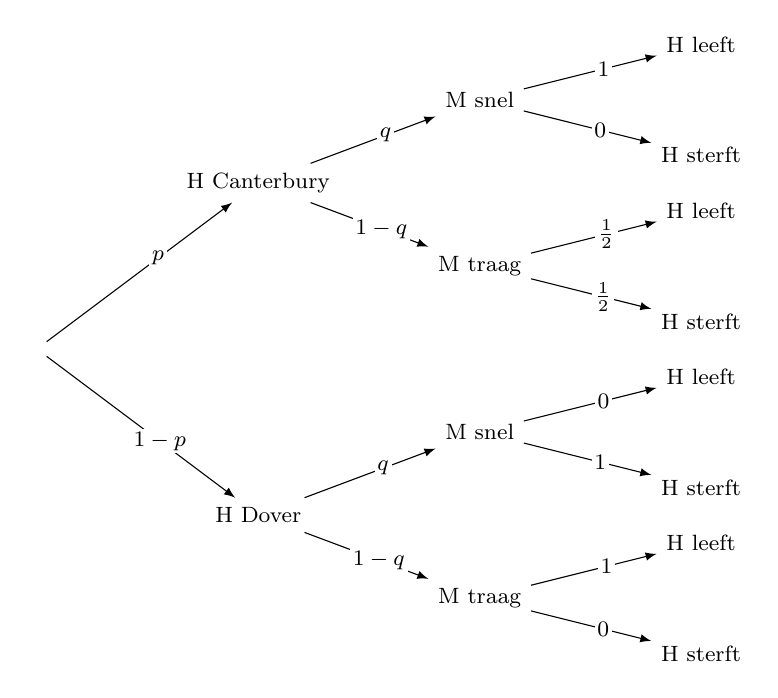
\begin{tikzpicture}[
  grow'=right,
  sibling distance=8em,
  level distance=8em,
  edge from parent/.style={draw, -latex},
  every node/.style={font=\footnotesize},
  level 1/.style={sibling distance=12em},
  level 2/.style={sibling distance=6em},
  level 3/.style={sibling distance=4em},
  edge label/.style={pos=0.6, fill=white, inner sep=1pt}
]

% Boomstructuur
\node (start) {}
  child {node {H Canterbury}
    child {node {M snel}
      child {node {H leeft} edge from parent node[edge label] {$1$}}
      child {node {H sterft} edge from parent node[edge label] {$0$}}
      edge from parent node[edge label] {$q$}
    }
    child {node {M traag}
      child {node {H leeft} edge from parent node[edge label] {$\frac{1}{2}$}}
      child {node {H sterft} edge from parent node[edge label] {$\frac{1}{2}$}}
      edge from parent node[edge label] {$1 - q$}
    }
    edge from parent node[edge label] {$p$}
  }
  child {node {H Dover}
    child {node {M snel}
      child {node {H leeft} edge from parent node[edge label] {$0$}}
      child {node {H sterft} edge from parent node[edge label] {$1$}}
      edge from parent node[edge label] {$q$}
    }
    child {node {M traag}
      child {node {H leeft} edge from parent node[edge label] {$1$}}
      child {node {H sterft} edge from parent node[edge label] {$0$}}
      edge from parent node[edge label] {$1 - q$}
    }
    edge from parent node[edge label] {$1 - p$}
  };

\end{tikzpicture}
}

\emph{Met deze kansboom vinden de leerlingen:}

$$P(\text{Holmes overleeft}) = p\cdot q\cdot 1 + p\cdot (1-q)\cdot \frac{1}{2}+(1-p) \cdot q \cdot 0 + (1-p)\cdot(1-q)\cdot 1.$$

Dit is inderdaad de formule uit de opgave.

\vraag{Schrijf deze uitdrukking in de vorm $ap+b$ waarbij $a$ en $b$ afhangen van $q$.} 
\antwoord{Deze uitdrukking is $\text{P}(\text{Holmes overleeft)}=\left(\frac{3}{2}q-\frac{1}{2}\right)p+(1-q).$}

\vraag{Sherlock Holmes wil zijn overlevingskans maximaliseren. Welke waarde van $p$ neemt Holmes best als $q=\frac{1}{2}$? En als $q=\frac{1}{6}$? En als $q=\frac{1}{3}$?}

\antwoord{Voor $q=\frac{1}{2}$ is is de overlevingskans van Holmes gelijk aan $\frac{1}{4}p+\frac{1}{2}$. Hij neemt dan best $p$ zo groot mogelijk, dus: $p=1$. Voor $q=\frac{1}{6}$ is de overlevingskans van Holmes gelijk aan $-\frac{1}{4}p+\frac{5}{6}$. Hij neemt dan best $p$ zo klein mogelijk, dus: $p=0$. Voor $q=\frac{1}{3}$ is is de overlevingskans van Holmes gelijk aan $0\cdot p+\frac{2}{3}=\frac{2}{3}$. Dan maakt het niet uit welke waarde van $p$ hij neemt.}
\vraag{ Voor welke waarden van $q$ moet hij $p=1$ nemen (en dus in Canterbury uitstappen) en voor welke waarden van $q$ neemt hij best $p=0$ (en rijdt hij best door tot Dover)?}

\antwoord{Als $q>\frac{1}{3}$ dan is de coëfficiënt van $p$ positief en is het voor Holmes interessant om $p$ zo groot mogelijk te nemen, dus $p=1$. In dat geval zal hij in Canterbury uitstappen. Als $q<\frac{1}{3}$, dan is de coëfficiënt van $p$ negatief en wil Holmes $p$ zo klein mogelijk nemen, dus $p=0$. In dat geval blijft hij zitten tot Dover. En voor $q=\frac{1}{3}$ maakt het niet uit want dan is de coëfficiënt van $p$ nul.}

\vraag{Moriarty wil de overlevingskans van Holmes minimaliseren. Hoe herschrijft hij de overlevingskans van Holmes? Voor welke waarden van $p$ neemt hij best de snelle trein en voor welke waarden van $p$ neemt hij best de trage trein?}

\antwoord{Hij schrijft de overlevingskans van Holmes in de vorm $aq+b$ waarbij $a$ en $b$ afhangen van $p$. Dit geeft:}

$$\text{P}(\text{Holmes overleeft)}=\left(\frac{3}{2}p-1 \right)q+\left(1-\frac{p}{2}\right).$$

\emph{Als $p>\frac{2}{3}$ is de coëfficiënt van $q$ positief. Omdat hij de overlevingskans van Holmes wil minimaliseren, neemt hij dan $q=0$, de trage trein dus. Als $p<\frac{2}{3}$, is de coëfficiënt van $q$ negatief en neemt hij $q=1$, de snelle trein. En als $p=\frac{2}{3}$ maakt het niet uit want dan is de coëfficiënt van $q$ nul.}

\end{vraagenantwoord}

De grafiek hieronder vat de strategieën van beide personages samen. Op de horizontale as is de kans $p$ uitgezet en op de verticale as de kans $q$. In het groen zie je de optimale waarde van $p$ in functie van $q$ en in het rood de optimale waarde van $q$ in functie van $p$.

\afbeelding[6.5cm]{img/Lspeltheorie/nash.png}{}{}

Het snijpunt $\left( \frac{2}{3}, \frac{1}{3}\right)$ is het zogenaamde \emph{Nash-evenwicht}. Van zodra Holmes afwijkt van $p=\frac{2}{3}$, kan zijn tegenstander zijn overlevingskans naar nul brengen door een geschikte keuze van $q$ (namelijk $1$ of $0$). Analoog kan Moriarty geen betere $q$-waarde nemen dan $\frac{1}{3}$, want anders kan Holmes een $p$-waarde nemen (namelijk $0$ of $1$) die hem met zekerheid doet ontsnappen.

Sherlock Holmes moet dus met kans $\frac{2}{3}$ in Canterbury uitstappen. Hij kan bv. een dobbelsteen gooien en als het aantal ogen $1, 2, 3$ of $4$ is, in Canterbury uitstappen. En Moriarty moet met kans $\frac{1}{3}$ de snelle trein nemen (bijvoorbeeld door een dobbelsteen te gooien en de snelle trein nemen als het aantal ogen $1$ or $2$ is).

\begin{vraagenantwoord}[resume]
\vraag{Wat is nu de overlevingskans van Holmes in het Nash-evenwicht?}

\antwoord{De evenwichtswaarden van $p$ en $q$ invullen in één van de uitdrukkingen voor zijn overlevingskans geeft: \emph{\text{P}(\text{Holmes overleeft)}}$=\frac{2}{3}$.}
\end{vraagenantwoord}
\end{lesactiviteit}\clearpage
\begin{multicols}{2}
\section{Penalty's}\label{sec:penalties}

In deze paragraaf bekijken we speltheorie in de context van het trappen van penalty's bij voetbalwedstrijden. We zien het trappen van een penalty als een spel met twee spelers waarbij de penaltytrapper steeds de rijspeler is en de keeper de kolomspeler. We bestuderen het vereenvoudigde model waarbij de penaltytrapper enkel links (L) of rechts (R) trapt en de keeper enkel links (L) of rechts (R) duikt. Belangrijke afspraak: als de penaltytrapper links kiest en de keeper ook (dus beiden L), dan bedoelen we dat de keeper naar de hoek duikt waar de bal terecht komt. We hanteren met andere woorden L en R altijd vanuit het perspectief van de trapper  (zie figuur \ref{fig:penalty09}).

\afbeelding{img/Lspeltheorie/penalty09.jpg}{Links (L) en rechts (R) trappen en duiken}{fig:penalty09}

Andere gevallen, zoals bijvoorbeeld de situatie dat een penaltytrapper de bal naar het midden van de goal trapt, laten we achterwege. We maken ook geen onderscheid tussen de bal over de grond trappen of in de winkelhaak enz., al zijn dat strategisch natuurlijk ook wel interessante keuzes.

Voor elke keuze die de spelers maken (bijvoorbeeld de penaltytrapper trapt naar links en de keeper duikt naar rechts), kunnen we met een kansentabel de verwachte winst of opbrengst voor elke speler berekenen. De trapper wil natuurlijk zoveel mogelijk doelpunten scoren terwijl de keeper zoveel mogelijk doeltrappen wil stoppen.

\subsection*{Voorbeeld 1}
We starten met de eenvoudige situatie waarbij de penaltytrapper altijd scoort als de keeper naar de verkeerde hoek duikt en de keeper de bal altijd pakt als hij naar de juiste hoek duikt. De bimatrix van deze situatie ziet er uit als volgt:
\begin{center}
    \begin{tabular}{c c c}
        & \hspace{0.4cm} \textbf{\textcolor{purple}{keeper}} & \\
        &\hspace{-0.4cm} L &\hspace{-1cm} R \\  
        \textbf{\textcolor{green}{penaltytrapper}} \begin{tabular}{c}
             L\\
             R
        \end{tabular} &  
        \multicolumn{2}{c}{$\left[ \begin{array}{cc} 
                    \textcolor{green}{0};\textcolor{purple}{1} & \textcolor{green}{1};\textcolor{purple}{0} \\ 
                    \textcolor{green}{1};\textcolor{purple}{0} & \textcolor{green}{0};\textcolor{purple}{1}  
                  \end{array} \right]$} 
    \end{tabular}
\end{center}

De getallen in de bimatrix stellen voor beide spelers de kansen voor op winst d.w.z. de kans op scoren voor de trapper (groen) en de kans op de penalty stoppen voor de keeper (rood). 

Stel dat de gemengde strategie van de penaltytrapper $\displaystyle \left(\frac{1}{3}, \frac{2}{3}\right)$ is. Dit betekent dat de penaltytrapper 1 op 3 penalty's links trapt en 2 op 3 rechts. Wat is nu de beste reactie van de keeper? Als de keeper links kiest, dan is zijn verwachte winst $\displaystyle 1\cdot \frac{1}{3}+0\cdot \frac{2}{3}=\frac{1}{3}$. Duikt de keeper rechts, dan is zijn verwachte winst $\displaystyle \frac{2}{3}$. We stellen dit schematisch voor:

\begin{center}
    \begin{tabular}{r c c}  
       \begin{tabular}{c}
            \textcolor{green}{$1/3$}\\
            \textcolor{green}{$2/3$}
        \end{tabular} &  
        \multicolumn{2}{c}{$\left[ \begin{array}{cc} 
                    \textcolor{green}{0};\textcolor{purple}{1} & \textcolor{green}{1};\textcolor{purple}{0} \\ 
                    \textcolor{green}{1};\textcolor{purple}{0} & \textcolor{green}{0};\textcolor{purple}{1}  
                  \end{array} \right]$}\\[0.5cm]                  
        winst keeper:&\ \ \ \textcolor{purple}{$1/3$}&\textcolor{purple}{$2/3$}   
    \end{tabular}
\end{center}

De keeper zal dus liever naar rechts duiken en zal in dit geval niet reageren met een gemengde strategie maar met een zuivere strategie namelijk altijd naar rechts duiken. Deze situatie is echter niet in evenwicht: als de keeper altijd rechts duikt, zal de penaltytrapper dit na zekere tijd door krijgen en zal hij zijn strategie veranderen en altijd links trappen. Daarop zal de keeper dan weer altijd links kiezen en dan de trapper altijd rechts, dus de keeper altijd rechts enz. Zuivere strategieën leiden in deze context tot een instabiele situatie.

Om te vermijden dat de keeper voordeel heeft bij een bepaalde keuze (links of rechts duiken) en reageert met een zuivere strategie, moet de trapper zijn gemengde strategie zó kiezen dat de winst voor de keeper gelijk blijft, of hij nu links duikt of rechts. Hoe vinden we die gemengde strategie voor de trapper?

Stellen we algemeen de gemengde strategie van de penaltytrapper gelijk aan $(1-p, p)$. De kans dat hij naar links trapt is dus $1-p$ en de kans dat hij naar rechts trapt $p$. Dan is de verwachte winst van de keeper $1-p$ bij duiken naar links en $p$ bij duiken naar rechts. Schematisch:
\begin{center}
    \begin{tabular}{r c c}  
       \begin{tabular}{r}
            \textcolor{green}{$1-p$}\\
            \textcolor{green}{$p$}
        \end{tabular} &  
        \multicolumn{2}{c}{$\left[ \begin{array}{cc} 
                    \textcolor{green}{0};\textcolor{purple}{1} & \textcolor{green}{1};\textcolor{purple}{0} \\ 
                    \textcolor{green}{1};\textcolor{purple}{0} & \textcolor{green}{0};\textcolor{purple}{1}  
                  \end{array} \right]$}\\[0.5cm]                  
        winst keeper:&\ \ \textcolor{purple}{$1-p$}&\ \ \textcolor{purple}{$p$}   
    \end{tabular}
\end{center}

We zoeken de gemengde strategie van de trapper die ertoe leidt dat de winst voor de keeper bij links duiken gelijk is aan de winst bij rechts duiken. We zoeken dus $p$ zo dat $1-p=p$, of nog $p=\frac{1}{2}$. De strategie van de trapper is dan $\displaystyle \textcolor{green}{\left(\frac{1}{2},\frac{1}{2} \right)}$. Met deze strategie maakt het niet uit welke kant de keeper kiest. Zowel bij duiken naar links als naar rechts is zijn winst $\frac{1}{2}$. Hij kan die winst niet verhogen.

Deze hele redenering is natuurlijk wederkerig. We wisselen het perspectief: stel dat de strategie van de keeper $(1-q, q)$ is. Wat is dan de reactie van de penaltytrapper? Als de trapper links trapt, dan is zijn verwachte winst $0\cdot (1-q)+1\cdot q=q$ en als hij rechts trapt, is zijn verwachte winst $1-q$. Zolang deze winsten ongelijk zijn, zal de trapper voordeel hebben bij een bepaalde keuze (links of rechts) en reageren met een zuivere strategie. Dit leidt, zoals hierboven beschreven, tot een situatie die niet in evenwicht is.

\begin{center}
    \begin{tabular}{r c c}  
       %\begin{tabular}{r}
        %    \textcolor{green}{$1-p$}\\
         %   \textcolor{green}{$p$}
        %\end{tabular} 
         \hspace{0.2 cm}\textcolor{purple}{$1-q$} & \hspace{-0.2 cm}\textcolor{purple}{$q$} & winst penaltytrapper\\
         \multicolumn{2}{c}{$\left[ \begin{array}{cc} 
                    \textcolor{green}{0};\textcolor{purple}{1} & \textcolor{green}{1};\textcolor{purple}{0}  \\ 
                    \textcolor{green}{1};\textcolor{purple}{0} & \textcolor{green}{0};\textcolor{purple}{1}
                  \end{array} \right]$}  & \begin{tabular}{l}
                                            \textcolor{green}{$q$}\\
                                            \textcolor{green}{$1-q$}
                                            \end{tabular}
    \end{tabular}
\end{center}


Om te vermijden dat de trapper voordeel heeft bij een bepaalde keuze moet de keeper zijn strategie zo kiezen dat $q=1-q$ of $q=\frac{1}{2}$. De verwachte winst van de trapper is dan zowel bij links als bij rechts trappen gelijk aan $\frac{1}{2}$. De strategie van de keeper is in dit geval $\displaystyle \textcolor{purple}{\left(\frac{1}{2},\frac{1}{2} \right)}$.

Conclusie: de combinatie van gemengde strategieën $\displaystyle \left( \textcolor{green}{\left(\frac{1}{2},\frac{1}{2} \right)},\textcolor{purple}{\left(\frac{1}{2},\frac{1}{2} \right)}  \right)$ is voor dit spel een evenwicht. De spelers wisselen hierbij random tussen links en rechts spelen. Dit evenwicht wordt een \textbf{Nash-evenwicht} genoemd. Geen van beide spelers kan er in dat geval op vooruit gaan door eenzijdig af te wijken van zijn strategie. Er is voor niemand een stimulans om te veranderen van strategie.

In 1949 bewees John Nash dat er voor ieder spel met $n$ spelers een evenwicht bestaat, dit is een strategieëncombinatie $(s_1, s_2\ldots s_n)$ waarbij geen enkele speler zich kan verbeteren door eenzijdig van strategie te veranderen.

%Hij dwingt de keeper zo tot een gemengde strategie en random wisselen tss links en rechts duiken volges de verdeling van die strategie.

\subsection*{Voorbeeld 2}
Bekijken we nu de iets complexere situatie waarbij de penaltytrapper minder goed rechts trapt dan in vorig voorbeeld. Hij mist daardoor in $25\%$ van de gevallen wanneer hij naar rechts trapt terwijl de keeper naar links duikt en het doel dus open ligt. De bimatrix wordt dan:
\begin{center}
    \begin{tabular}{c c c}
        & \hspace{1.2 cm}\textbf{\textcolor{purple}{keeper}} & \\
        & L &\hspace{-0.7cm} R \\  
        \textbf{\textcolor{green}{penaltytrapper}} \begin{tabular}{c}
             L\\
             R
        \end{tabular} &  
        \multicolumn{2}{c}{$\left[ \begin{array}{cc} 
                    \textcolor{green}{0};\textcolor{purple}{1} & \textcolor{green}{1};\textcolor{purple}{0} \\ 
                    \textcolor{green}{0,75};\textcolor{purple}{0,25} & \textcolor{green}{0};\textcolor{purple}{1}  
                  \end{array} \right]$} 
    \end{tabular}
\end{center}
De interpretatie van de getallen in de bimatrix blijft hetzelfde. Als de penaltytrapper naar rechts trapt en de keeper duikt naar links dan is de kans op winst voor de trapper, dit is de kans op scoren, gelijk aan $75\%$. Merk op dat dit tegelijk de kans is op verlies voor de keeper. De kans op winst voor de keeper, met andere woorden de kans dat er niet wordt gescoord, is dan $25\%$. Dit is ook de kans op verlies voor de trapper. 



Wat is nu het nieuwe evenwicht?

In vorig voorbeeld zochten we eerst de strategie van de trapper in het Nash-evenwicht. Het maakt niet uit met welke speler je begint. We beginnen hier met de keeper. Stel opnieuw de strategie van de keeper voor door $(1-q, q)$. Als de penaltytrapper links trapt, is zijn verwachte winst $0\cdot (1-q)+1\cdot q=q$. Trapt hij rechts dan is zijn verwachte winst $0,75\cdot (1-q)+0\cdot q=-0,75q+0,75$.

\begin{center}
    \begin{tabular}{r c c}  
       %\begin{tabular}{r}
        %    \textcolor{green}{$1-p$}\\
         %   \textcolor{green}{$p$}
        %\end{tabular} 
         \hspace{0.5 cm}\textcolor{purple}{$1-q$} & \textcolor{purple}{$q$} & winst penaltytrapper\\
         \multicolumn{2}{c}{$\left[ \begin{array}{cc} 
                    \textcolor{green}{0};\textcolor{purple}{1} & \textcolor{green}{1};\textcolor{purple}{0}  \\ 
                    \textcolor{green}{0,75};\textcolor{purple}{0,25} & \textcolor{green}{0};\textcolor{purple}{1}
                  \end{array} \right]$}  & \begin{tabular}{l}
                                            \textcolor{green}{$q$}\\
                                            \textcolor{green}{$-0,75q+0,75$}
                                            \end{tabular}
    \end{tabular}
\end{center}

Zolang de penaltytrapper voordeel heeft bij een bepaalde keuze (links of rechts trappen) zal hij op de gemengde strategie van de keeper reageren met een zuivere strategie. Om dat te vermijden moet de strategie van de keeper zo zijn dat het mogelijke voordeel voor de trapper wegvalt. De keeper moet er met andere woorden voor zorgen dat het voor de trapper niet uitmaakt hoe hij trapt (links of rechts). Dit is zo als de verwachte winst van de penaltytrapper bij links trappen gelijk is aan de verwachte winst bij rechts trappen of nog als  $q=-0,75q+0,75$. Hieruit vinden we: $\displaystyle q=\frac{3}{7}\approx 0,43$. Dit leert ons dat de keeper in 4 van de 7 gevallen links moet duiken en in 3 van de 7 rechts. De strategie van de keeper is $\displaystyle \textcolor{purple}{\left(\frac{4}{7}, \frac{3}{7}\right)}$. Zowel bij trappen naar links als naar rechts
is de verwachte winst van de penaltytrapper dan gelijk aan $\frac{3}{7}$. In deze situatie zal de trapper voor een gemengde strategie kiezen. Hij kan zich niet verbeteren door voor een zuivere strategie te kiezen.

We kunnen deze situatie grafisch interpreteren als het snijpunt van de twee rechten die de verwachte winst (als functie van $q$) voorstellen van de penaltytrapper bij links of rechts trappen (zie figuur \ref{fig:penalty01}). Je herkent in deze figuur in groen de elementen uit de kolommen van de bimatrix voor de penaltytrapper.

We doen nog een andere interessante vaststelling: $\displaystyle \textcolor{purple}{\left(\frac{4}{7}, \frac{3}{7}\right)}$ is een minimax-strategie. Op de gemengde strategie van de keeper zal de trapper steeds reageren door te kiezen voor de strategie die hem maximale winst oplevert, d.w.z. zoveel mogelijk goals. De keeper moet bijgevolg kiezen voor de strategie die de maximale winst voor de trapper minimaliseert. Hij minimaliseert in dat geval het verlies dat hijzelf hoogstens kan hebben. De grafiek die de maximale winst voor de trapper aangeeft, is in blauw getekend in figuur \ref{fig:penalty01}. Het snijpunt is het punt waar die maximale minst zo klein mogelijk is. De strategie die erbij hoort, is dus een minimax-strategie.

\afbeelding[0.8\textwidth]{img/Lspeltheorie/penalty01.jpg}{Verwachte winsten van de penaltytrapper (als hij links of rechts trapt) in functie van $q$. In het snijpunt zijn deze winsten gelijk en maakt het niet uit hoe hij trapt.}{fig:penalty01}


Bekijken we nu wat de penaltytrapper moet doen. De redenering is helemaal analoog. We stellen de strategie van de penaltytrapper $(1-p,p)$ en zoeken de waarde van $p$ waarvoor het niet uitmaakt wat de keeper doet. Als de keeper links kiest, dan is zijn verwachte winst $1\cdot (1-p)+0,25\cdot p=1-0,75p$. Duikt hij rechts dan is dat $0\cdot (1-p)+1\cdot p=p$.

\begin{center}
    \begin{tabular}{r c c}  
       \begin{tabular}{r}
            \textcolor{green}{$1-p$}\\
            \textcolor{green}{$p$}
        \end{tabular} &  
        \multicolumn{2}{c}{$\left[ \begin{array}{cc} 
                    \textcolor{green}{0};\textcolor{purple}{1} & \textcolor{green}{1};\textcolor{purple}{0} \\ 
                    \textcolor{green}{0,75};\textcolor{purple}{0,25} & \textcolor{green}{0};\textcolor{purple}{1}  
                  \end{array} \right]$}\\[0.5cm]                  
        winst keeper:&\ \ \textcolor{purple}{$1-0,75p$}&\ \ \textcolor{purple}{$p$}   
    \end{tabular}
\end{center}

De trapper moet er met zijn strategie voor zorgen dat de keeper geen voordeel kan doen bij de ene of de andere keuze (links of rechts duiken). Dit is zo als de verwachte winsten voor de keeper gelijk zijn, of nog als $1-0,75p=p$. We vinden dan: $\displaystyle p=\frac{4}{7}\approx 0,57$. De trapper moet dus in $4$ van de $7$ gevallen naar rechts trappen. Zijn strategie wordt $\displaystyle \textcolor{green}{\left(\frac{3}{7}, \frac{4}{7}\right)}$. De grafische interpretatie van deze situatie (als snijpunt van twee rechten) wordt getoond in figuur \ref{fig:penalty02}. 

We kunnen opnieuw grafisch inzien dat hier een minimax-strategie wordt gespeeld. De penaltytrapper zal voor de strategie kiezen die de maximale winst voor de keeper minimaliseert. Hij minimaliseert hiermee het verlies dat hijzelf hoogstens kan verwachten. De grafiek die de maximale verwachte winst voor de keeper aangeeft, is in blauw getekend in figuur \ref{fig:penalty02}. Het snijpunt is het punt waar die maximale winst zo klein mogelijk is.

\afbeelding[0.8\textwidth]{img/Lspeltheorie/penalty02.jpg}{Verwachte winsten van de keeper (als hij links of rechts duikt) in functie van $p$. In het snijpunt zijn deze winsten gelijk en maakt het niet uit hoe de keeper duikt.}{fig:penalty02}

Conclusie: het Nash-evenwicht is de combinatie van de minimax-strategieën $\displaystyle \left( \textcolor{green}{\left(\frac{3}{7},\frac{4}{7} \right)},\textcolor{purple}{\left(\frac{4}{7},\frac{3}{7} \right)}  \right)$. De spelers wisselen hierbij random tussen links en rechts volgens de verdeling uit het evenwicht. Geen van beide spelers kan zich in die situatie verbeteren door eenzijdig van strategie te veranderen.

We kunnen ons de vraag stellen wie in het voordeel is bij dit evenwicht. De kans dat er gescoord wordt, dit is de kans dat de penaltytrapper wint, is: $$1\cdot \frac{3}{7}\cdot \frac{3}{7}+0,75\cdot \frac{4}{7}\cdot \frac{4}{7}=\frac{3}{7}.$$ De keeper is licht in het voordeel: de kans dat er niet gescoord wordt en de keeper wint, is $\frac{4}{7}$. Je ziet hier het effect van de minder goede rechtertrap van de penaltytrapper. 

Dat de penaltytrapper in dit Nash-evenwicht vaker rechts zal trappen hoewel dit zijn zwakke kant is, lijkt misschien contradictorisch. Dat komt omdat de keeper zich ook heeft aangepast. Als de keeper nog, zoals in voorbeeld 1, strategie $\displaystyle \left(\frac{1}{2},\frac{1}{2}\right)$ zou aannemen, dan zou de penaltytrapper altijd naar links trappen. Hij zou dan geen nadeel ondervinden van zijn zwakkere rechterkant en de helft van de tijd scoren. Door vaker naar links te duiken, forceert de keeper de trapper om toch naar zijn zwakke rechterkant te trappen en kan hij de kans op een goal verminderen van $\frac{1}{2}$ naar $\frac{3}{7}$.

Het Nash-evenwicht is hier de combinatie van de minimax-strategieën.
Binnen speltheorie is aangetoond dat dit altijd zo is bij een nulsomspel met twee spelers. Het echter niet zo dat een Nash-evenwicht altijd samenvalt met de minimax-strategieën.
% Een uitnodigende vraag voor de lezer om meer in de wiskundige theorie te duiken: zou het penalty trappen een ``nul''somspel genoemd kunnen worden?

Na deze twee voorbeelden kunnen we begrijpen wat het in de praktijk betekent om gemengde strategieën te spelen volgens een Nash-evenwicht. Beide spelers randomiseren hun spel om zo de tegenspeler in de war te brengen en de eigen acties onvoorspelbaar te maken. Moest de tegenspeler immers wél zeker weten wat een speler doet, dan zou hij daar voordeel uit halen en met een zuivere strategie (dus voorspelbaar) reageren waarop de andere speler op zijn beurt zal reageren met een zuivere strategie enzovoort. De spelers moeten een mate van onzekerheid hebben over elkaars acties.

\subsection*{De werkelijke situatie}
We vragen ons nu af of dit Nash-evenwicht in de praktijk waarneembaar is. Spelen spelers op groepsniveau zoals het Nash-evenwicht voorspelt? Randomiseren ze tussen links en rechts trappen of duiken? Palacios-Heurta  (2003) verzamelde data over maar liefst 1417 penalty's uit allerlei FIFA-wedstrijden in Spanje, Engeland, Italië … Hij deelde de doeltrappen op in links, midden en rechts en ging o.a. na met welk been een penalty werd getrapt. Dat laten wij hier buiten beschouwing. Uit zijn waarnemingen kunnen we wel de relevante data afleiden voor onze bespreking. Op basis van de steekproef van 1417 penalty's vinden we de volgende bimatrix:

\begin{center}
    \begin{tabular}{c c c}
        & \hspace{1.5 cm}\textbf{\textcolor{purple}{keeper}} & \\
        & L &\hspace{-0.5cm} R \\  
        \textbf{\textcolor{green}{trapper}} \begin{tabular}{c}
             L\\
             R
        \end{tabular} &  
        \multicolumn{2}{c}{$\left[ \begin{array}{cc} 
                    \textcolor{green}{0,58};\textcolor{purple}{0,42} & \textcolor{green}{0,95};\textcolor{purple}{0,05} \\ 
                    \textcolor{green}{0,93};\textcolor{purple}{0,07} & \textcolor{green}{0,70};\textcolor{purple}{0,30}  
                  \end{array} \right]$} 
    \end{tabular}
\end{center}

Hoe moeten we deze cijfers interpreteren?
Wanneer een penaltytrapper naar links trapt en de keeper naar links duikt dan wint (d.w.z. scoort) de trapper gemiddeld gezien in $58\%$ van de gevallen en wint de keeper (d.w.z. er wordt niet gescoord) gemiddeld gezien in $42\%$ van de gevallen. Deze percentages zijn gebaseerd op de 1417 penalty's. Het zijn empirische kansen.

Wat valt op in deze matrix? Als de keeper de verkeerde kant kiest, wordt er iets meer gescoord bij de linkse trappen dan bij die naar rechts. Misschien zijn er meer rechtsvoetige penaltytrappers en voor rechtsvoetigen zijn trappen naar links iets natuurlijker. Dat effect is weliswaar bij professionele voetballers bijna volledig weggewerkt.

Verder zien we ook: als de keeper dezelfde kant kiest als de kant waarnaar getrapt wordt, dan is naar rechts trappen duidelijk beter. De verklaring is misschien dat bij trappen naar rechts de keeper op zijn eigen linkerzijde moet duiken. Dat is minder natuurlijk voor rechtshandige keepers en dus wellicht een stuk moeilijker. Het effect van spelen met je minder natuurlijke kant lijkt bij keepen zwaarder door te wegen dan bij trappen.

Om het Nash-evenwicht te zoeken voor deze situatie, maken we de gebruikelijke schema's.

We zoeken eerst de strategie van de keeper. Wat moet hij doen?
\begin{center}
    \begin{tabular}{r c c}  
       %\begin{tabular}{r}
        %    \textcolor{green}{$1-p$}\\
         %   \textcolor{green}{$p$}
        %\end{tabular} 
         \textcolor{purple}{$\ \ \ \ \ \ \ 1-q$} & \textcolor{purple}{$q$} & winst trapper\\
         \multicolumn{2}{c}{$\left[ \begin{array}{cc} 
                    \textcolor{green}{0,58};\textcolor{purple}{0,42} & \textcolor{green}{0,95};\textcolor{purple}{0,05} \\ 
                    \textcolor{green}{0,93};\textcolor{purple}{0,07} & \textcolor{green}{0,70};\textcolor{purple}{0,30} 
                  \end{array} \right]$}  & \begin{tabular}{l}
                                            \textcolor{green}{$0,37q+0,58$}\\
                                            \textcolor{green}{$-0,23q+0,93$}
                                            \end{tabular}
    \end{tabular}
\end{center}

De waarschijnlijkheid van links duiken $(1-q)$ of rechts duiken $(q)$ moet zo zijn dat het niet uitmaakt wat de penaltytrapper doet (zoniet reageert die met een zuivere strategie). De winsten moeten dus hetzelfde zijn, of de trapper nu met links of rechts trapt. Dus moet: $$0,37q+0,58=-0,23q+0,93.$$ Hieruit volgt $\displaystyle q= \frac{7}{12}$. De strategie die de keeper moet volgen, is $\displaystyle \textcolor{purple}{\left(\frac{5}{12}, \frac{7}{12}\right)}$. De verwachte winst voor de trapper is dan altijd gelijk aan $0,37\cdot \frac{7}{12}+0,58\approx 0,80$, hoe hij ook trapt.

In figuur \ref{fig:penalty03} zie je de visualisering van deze situatie. Merk hier opnieuw op dat de keeper bij deze strategie zijn maximaal verwachte verlies zo klein mogelijk maakt. De strategie die de keeper zal volgen, is een minimax-strategie.

\afbeelding[0.8\textwidth]{img/Lspeltheorie/penalty03.jpg}{Verwachte winsten van de penaltytrapper (als hij links of rechts trapt) in functie van $q$. In het snijpunt zijn deze winsten gelijk en maakt het niet uit hoe er getrapt wordt.}{fig:penalty03}

Wat moet de penaltytrapper doen? We kennen ondertussen de procedure: de strategie van de penaltytrapper moet zo zijn dat het niet uitmaakt wat de keeper doet. De winsten van de keeper moeten gelijk zijn.
\begin{center}
    \begin{tabular}{r c c}  
       \begin{tabular}{r}
            \textcolor{green}{$1-p$}\\
            \textcolor{green}{$p$}
        \end{tabular} &  
        \multicolumn{2}{c}{$\left[ \begin{array}{cc} 
                    \textcolor{green}{0,58};\textcolor{purple}{0,42} & \textcolor{green}{0,95};\textcolor{purple}{0,05} \\ 
                    \textcolor{green}{0,93};\textcolor{purple}{0,07} & \textcolor{green}{0,70};\textcolor{purple}{0,30}  
                  \end{array} \right]$}\\[0.5cm]                  
        winst keeper:&\ \ \textcolor{purple}{\hspace{-0.2cm}$-0,35p+0,42$}&\ \ \textcolor{purple}{\hspace{-0.2cm}$0,25p+0,05$}   
    \end{tabular}
\end{center}
Dus moet $-0,35p+0,42=0,25p+0,05$. Hieruit vinden we $\displaystyle p=\frac{37}{60}$. De strategie van de penaltytrapper is  $\displaystyle \textcolor{green}{\left(\frac{23}{60}, \frac{37}{60}\right)}$ en de verwachte winst voor de keeper is $-0,35\cdot \frac{37}{60}+0,42\approx 0,20$.
\vfill\null
\columnbreak
Conclusie: het Nash-evenwicht is de combinatie van de twee gevonden strategieën $\displaystyle \left( \textcolor{green}{\left(\frac{23}{60},\frac{37}{60} \right)},\,\textcolor{purple}{\left(\frac{5}{12},\frac{7}{12} \right)}  \right)$ of nog $\displaystyle \left( \textcolor{green}{\left(0,38; 0,62 \right)},\,\textcolor{purple}{\left(0,42;0,58 \right)}  \right)$. Beide spelers wisselen hierbij random tussen links en rechts spelen volgens deze verdelingen. Dit zijn ook de minimax-strategieën voor beide spelers. Uit de verwachte winsten van elke speler ($0,80$ voor de trapper en dus $0,20$ voor de keeper) leiden we af dat de trapper sterk in het voordeel is in deze situatie.

Zien we dit evenwicht terug in de waargenomen data over de echte strafschoppen in het onderzoek? In het onderzoek van Palacios-Heurta wordt getoond dat spelers inderdaad randomiseren tussen links en rechts trappen of duiken. In figuur \ref{fig:penalty04} vergelijken we de waargenomen frequenties met de theoretische Nash-frequenties die we net berekend hebben op basis van de bimatrix met de empirische kansen. We weten bijvoorbeeld dat penaltytrappers in $38\%$ van de gevallen links zouden moeten trappen volgens de voorspellingen bij het Nash-evenwicht. Dit komt goed overeen met de waarnemingen: bij de 1417 onderzochte penalty's wordt er in $40\%$ van de gevallen naar links getrapt bij een penalty enz. 

\afbeelding[0.8\textwidth]{img/Lspeltheorie/penalty04.jpg}{Vergelijking van de berekende Nash-frequenties met de waargenomen frequenties uit de steekproef.}{fig:penalty04}

De overeenkomsten zijn duidelijk: professionele voetbalspelers spelen op groepsniveau blijkbaar bijna perfect volgens de gemengde minimax-strategieën bij het Nash-evenwicht!
\end{multicols}

\afbeelding[0.5\textwidth]{img/loep-nashevenwichtgoal.jpg}{}{}\clearpage
\begin{multicols}{2}
\section{Pioniers: John von Neumann en John Nash}\label{sec:pioniers}

Speltheorie is als discipline ontstaan in de jaren 1920. Eén van de grondleggers is de Hongaars-Amerikaanse wiskundige John von Neumann (1903–1957).

\afbeelding[0.6\linewidth]{img/Lspeltheorie/penalty10.jpg}{John von Neumann}{fig:penalty10}

In 1928 publiceerde von Neumann het artikel ``Zur Theorie der Gesellschaftsspiele'' waarin hij de minimax-stelling formuleerde. Dit werk was belangrijk voor de ontwikkeling van speltheorie als op zichzelf staande discipline omdat het bewees dat strategisch gedrag wiskundig te modelleren valt. De grote doorbraak kwam in 1944 toen von Neumann samen met de Oostenrijkse econoom Oskar Morgenstern het invloedrijke boek ``Theory of Games and Economic Behavior'' publiceerde. Dit werk legde de wiskundige basis voor de toepassing van speltheorie in de economie en sociale wetenschappen. Het maakte de theorie bekend buiten de zuiver wiskundige wereld. The New York Times wijdde er zelfs een voorpaginaverhaal aan, een eer die tot dan toe alleen Einstein was te beurt gevallen.

John von Neumann groeide op in Boedapest in een Joods middenklassegezin. Hij studeerde wiskunde aan de universiteiten van Boedapest en Berlijn. Nadat hij voor het nazi-regime naar de Verenigde Staten was gevlucht, kwam hij terecht in Princeton, waar hij samen met Albert Einstein en Kurt Gödel een van de eerste hoogleraren werd aan het Institute for Advanced Study. Von Neumann was een opvallende figuur. Hij was een extravert levensgenieter die hield van snelle auto's, eten, drinken, dansen en plezier maken. Hij genoot ervan regelmatig grote feesten te geven in zijn huis in Princeton. Hij was niet alleen een genie in de wiskunde, maar leverde ook belangrijke bijdragen aan computerwetenschappen, natuurkunde en economie. Hij speelde een cruciale rol in de ontwikkeling van de computer. De zogenaamde von Neumann-architectuur vormt nog steeds de basis van de meeste moderne computersystemen. Tijdens de Tweede Wereldoorlog kwam hij terecht bij het Manhattanproject, waar hij meewerkte aan de ontwikkeling van de atoombom. Later was hij een sleutelfiguur in het opstellen van militaire strategieën tijdens de Koude Oorlog en adviseerde hij de Amerikaanse overheid over nucleaire wapens en raketsystemen. Von Neumann wordt als een van de meest invloedrijke wetenschappers ooit gezien.

In de jaren 1950 bouwde de Amerikaanse wiskundige John Nash (1928-2015) in de speltheorie voort op het werk van voorgangers zoals von Neumann.

John Forbes Nash jr werd in 1928 geboren in West Virginia en toonde al op jonge leeftijd uitzonderlijke wiskundige talenten. Na zijn studie aan het Carnegie Institute of Technology promoveerde hij in 1950 aan Princeton University met een proefschrift over speltheorie van slechts 27 pagina’s lang. Daarin introduceerde hij een 
revolutionair concept dat later bekend zou worden als het Nash-evenwicht. Dit maakte de speltheorie toepasbaar op een breder scala aan situaties, ook bij spellen waarin samenwerkingen tussen spelers mogelijk zijn.

\afbeelding[0.6\linewidth]{img/Lspeltheorie/penalty11.jpg}{John Nash}{fig:penalty11}

De ideeën uit Nash's proefschrift vormden de wiskundige ruggengraat van veel moderne economische theorieën. Hij werd voor dit werk in 1994 dan ook erkend met de Nobelprijs voor de economie (die hij deelde met John Harsanyi en Reinhard Selten).

John Nash leverde ook belangrijke bijdragen aan de algebraïsche meetkunde, differentiaalmeetkunde en theorie van partiële differentiaalvergelijkingen. Helaas werd zijn carrière lange tijd onderbroken door zijn decennialange strijd met schizofrenie. Hij maakte een opmerkelijke terugkeer naar de academische wereld in de jaren 1980 en kreeg later wereldwijde bekendheid door de film A Beautiful Mind (2001), gebaseerd op zijn leven. In 2015 ontving hij (samen met Louis Nirenberg) de prestigieuze Abelprijs voor zijn werk aan niet-lineaire partiële differentiaalvergelijkingen en toepassingen daarvan in complexe analyse en meetkunde. Hij  was de eerste persoon aan wie zowel een Nobelprijs als de Abelprijs werd toegekend. John Nash overleed in 2015, samen met zijn vrouw Alicia, bij een auto-ongeluk in New Jersey.

Nadat de ideeën van Nash de speltheorie breed toepasbaar maakten op talloze echte contexten, zoals financiële markten, onderhandelingen en conflicten, werden vanaf de jaren 1960 de concepten steeds verder uitgebreid en uitgediept door wiskundigen en economen zoals Reinhard Selten, John Harsanyi, Alvin Roth en Lloyd Shapley. Speltheorie is tegenwoordig een essentieel instrument in veel vakgebieden zoals economie, sociologie, bestuurskunde, milieubeleid, biologie …

Tot slot merken we op dat speltheorie beperkingen heeft en dat bijgevolg voorzichtig moet omgesprongen worden met de resultaten en modellen. In speltheorie wordt bijvoorbeeld meestal verondersteld dat spelers volledig rationeel zijn: ze kennen alle opties en uitkomsten, ze kunnen perfecte strategieën berekenen, ze handelen consequent … In werkelijkheid echter zijn mensen slechts beperkt rationeel, maken ze fouten of worden ze beïnvloed door emoties, gewoontes of sociale normen. Speltheorie is het meest effectief in situaties met duidelijke regels, een beperkt aantal spelers en helder gedefinieerde strategieën.
\stopcontents[inhoudloep]		% om inhoud voor het loep artikel te eindigen
\end{multicols}

\begin{bronnen}
    \item Case, N. (2017). \emph{The evolution of trust.} \url{ncase.me/trust} (App om herhaaldelijk een spel te spelen dat neerkomt op de gevangenenparadox)

    \item Chen, J., Lu, S., \& Vekhter, D. (z.d.). \emph{Von Neumann and the Development of Game Theory}. Game Theory. Geraadpleegd op 15 april 2025, van \url{https://cs.stanford.edu/people/eroberts/courses/soco/projects/1998-99/game-theory/index.html}
    
    \item{Chomp op \url{https://en.wikipedia.org/wiki/Chomp}}

    \item{Numberphile. (2013). \emph{Connect Four} op \url{https://www.youtube.com/watch?v=yDWPi1pZ0Po}}
    
    \item{Doyle, A. C. (1984). \emph{The final problem.} Penguin Books. (Oorspronkelijk gepubliceerd in 1893)}

    \item Jackson, M., Leyton-Brown, K., \& Shoham, Y. (2017, 13 juli). \emph{Game Theory Online}.\\ Geraadpleegd op 15 april 2025, van \url{https://www.game-theory-class.org/}
    
    \item{Krapf R. (4 april 2025). \emph{Determiniteit van (on)eindige spellen: Wanneer bestaat er een winnende strategie?}. Workshop op de Nationale Wiskunde Dagen in Noordwijkerhout.} \\ \url{chrome-extension://efaidnbmnnnibpcajpcglclefindmkaj/https://www.uu.nl/sites/default/files/Regula%20Krapf.pdf}
    
    \item Mr. Chadd (s.d.). \emph{Speltheorie.} \url{http://www.mrchadd.nl/academy/vakken/economie/speltheorie}

    \item O'Connor, J., \& Robertson, E. (2003). \emph{John von Neumann}. MacTutor Index.\\ Geraadpleegd op 15 april 2025, van \url{https://mathshistory.st-andrews.ac.uk/Biographies/Von_Neumann/}

    \item O'Connor, J., \& Robertson, E. (2015). \emph{John Forbes Nash}. MacTutor Index.\\ Geraadpleegd op 15 april 2025, van \url{https://mathshistory.st-andrews.ac.uk/Biographies/Nash/}
    
    \item Palacios-Heurta, I. (2003). Professionals play minimax. \emph{Review of Economic Studies.} vol. 70, 395-415.
    
    \item Scam Nation (s.d.). \emph{The big Tic Tac Toe prediction}. \url{http://www.youtube.com/watch?v=nqeAessIESU} (Goocheltoer over OXO gebaseerd op een idee van Martin Gardner)

    \item \emph{Speltheorie. Internationaal wiskundetoernooi 2024. Voorbereidend materiaal.} Universität Bonn, Leibniz Universität Hannover, KU Leuven, Radboud Universiteit Nijmegen. \\
    \url{http://www.ru.nl/sites/default/files/2024-09/voorbereidend-materiaal-wiskundetoernooi-2024.pdf}

    \item Terwijn, S. (2010). De Minimax-Stelling en Nash-Evenwichten. Nijmegen: Radboud Universiteit. \url{https://www.math.ru.nl/~terwijn/teaching/minimax.pdf}

    \item \emph{The game's afoot! Internationaal wiskundetoernooi 2024. Opgaven Sum of Us.}

    \item Thuijsman, F. (28 augustus 2020). \emph{Inleiding Speltheorie I, Niet-Coöperatieve Spelen.} Workshop Vakantiecursus 2020, Platform Wiskunde Nederland. \\ \url{https://www.platformwiskunde.nl/wp-content/uploads/2020/09/Syllabus-VC2020_v1.0.pdf}
    
    \item Thomas, R. (2012). \emph{Does it pay to be nice? - the maths of altruism.} \\
    \url{https://plus.maths.org/content/does-it-pay-be-nice-maths-altruism-part-i}

    \item Van Damme, E. (1995). Speltheorie, wiskunde van het strategisch handelen. \emph{Nieuwe Wiskrant 15/1}, 27-32.\\
    \url{https://www.fisme.science.uu.nl/wiskrant/artikelen/artikelen11-20/151/151september_vandamme.pdf}

	\item Watson, B. (2024). \emph{The beautiful game (theory) of why penalty takers ignore statistics.}\\
    \url{https://plus.maths.org/content/beautiful-game-theory-why-penalty-takers-ignore-statistics}
   
     \item \url{https://www.youtube.com/watch?v=yM38mRHY150} (split or steal)

    \item \url{https://www.youtube.com/watch?v=S0qjK3TWZE8} (split or steal: verrassende wending)
    
    \item \url{https://www.youtube.com/watch?v=wdDF7_vfLcE} (23 resultaten boter-kaas-en-eieren op symmetrie na)    
	
\end{bronnen}
